% Remove the /draft command in front of /begin{document} for final print!!!!
% and set the draft to false later on
% Ubuntu Precise related changes suggested by Heiko 06/21/2013
% --------------------------------------
%\documentclass[a4paper,12pt,american,draft]{book}
\documentclass[a4paper,12pt,american,final]{book}
\special{papersize=210mm,297mm}
\usepackage{a4}
\usepackage[pdftex]{geometry}
% --------------------------------------
\usepackage{advdate}%\SetDate[07/08/2017] % Set date in \today

\usepackage{tabularx,longtoc,booktabs,multirow}
\usepackage{textcomp}
%\usepackage[latin9]{inputenc}
\usepackage{times}
\usepackage[T1]{fontenc}              % Fonts with real
\usepackage{subscript}
\usepackage{color}
\usepackage{babel}% other languages/letters
\usepackage{afterpage}
%\usepackage{varioref}                 % pages in refs
\usepackage{graphics}                  % \usepackage[dvips]{graphics} for latex+dvips+ps2pdf
%\usepackage{graphicx}                 % \usepackage[dvips]{graphicx} for latex+dvips+ps2pdf
\usepackage{epsfig}                    % Enhanced PostScript (needed for SR tables!!!)
\usepackage{float}                     % exact positioning of floats ([H])
%\usepackage{floatfig}
\usepackage{wrapfig}
\usepackage{subfigure}                 % several pics, one title
%FAILED \usepackage{subcaption}                % DS supercedes subfigure. Used in Condensables
\usepackage{hyperref}                  % \href for emails or urls
%\usepackage{rotating}
\usepackage{array}                     % length \extrarowhheight fuer Tabellen
%\usepackage{supertabular}             % long tabels, pagewise
\usepackage{longtable}                 % long table, complete
\usepackage{threeparttable}
\usepackage[normalem]{ulem}            % sout.. needed by \DEL
%\usepackage{dcolumn}                  % table-values oriented to .
%\newcolumntype{d}[1]{D{.}{.}{#1}}
\usepackage{amsmath}
\usepackage{ifthen}                   % \ifthenelse command
\usepackage{xspace}                   % adds space only when needed
\usepackage[version=3]{mhchem}        % chemical molecular formulae, e.g. \ce{H2O}
%\usepackage{fancyhdrs}               % old version of fancyheadings
\usepackage{fancyhdr}                 %  Works with texlive
%DAVE \usepackage{fancyheadings}                  % special header
%\usepackage{portland}
%ds2004 \bibliographystyle{jacbib}
\usepackage[sectionbib]{natbib}
\bibpunct{(}{)}{,}{a}{}{,}   %For Patrick Daly's natbib package. In preamble
\usepackage{chapterbib}                % Bib after each chapter
%\usepackage{bibunits}                 % Bib after each chapter
\bibliographystyle{copernicus}         % change bibliography-name after each
\renewcommand\bibname{References}      % bibliographystyle command!

%Added by Dave:
%\usepackage[hyphens]{url}              % fro web-addresses
\usepackage[hyphens]{xurl} 
\usepackage{hyperref}                  % clickable cross-references and hyperlinks
\hypersetup{colorlinks=false,pdfborder={0 0 0},} % Remove ugly borders around hyperlinks
\usepackage[hyphenbreaks]{breakurl}
\usepackage[Sonny]{fncychap}
\usepackage{psfrag}
%\usepackage[Lenny]{fncychap}
%\usepackage[Glenn]{fncychap}
%\usepackage[Bjarne]{fncychap}
%added by Dave, 2005:
\usepackage{ccaption}
%added by Dave, 2006:
\usepackage{lscape}
%HM 2010
\usepackage[font=small]{caption}      % sets caption font and stile
\usepackage{doi}
\usepackage{tcolorbox}
%added by michaelS
\usepackage[percent]{overpic}
\usepackage{enumitem}

%Added by Agnes 09 July 2010
%Bigger text area on pages
%Page size redefined
\setlength{\textwidth}{15.7cm}
\setlength{\textheight}{24cm}
\setlength{\topmargin}{-1cm}
\setlength{\evensidemargin}{-5pt}

%
% Place for rule under heading
%
\addtolength{\headheight}{3pt}
\addtolength{\headsep}{-3pt}
%%%
%\newcommand{\Dave}[1]{{\color{red}{#1}}}

\newcommand{\DraftNote}[2]{\ifthenelse{\boolean{draftactive}}{\textcolor{#1}{#2}}{}}
\newcommand{\NEW}[1]{\DraftNote{red}{#1}}
\newcommand{\DEL}[1]{\DraftNote{green}{\sout{#1}}}
\newcommand{\QUERY}[1]{\DraftNote{magenta}{#1}}
\newcommand{\DAVE}[1]{\DraftNote{blue}{#1}}
\newcommand{\COMMENT}[1]{\DraftNote{cyan}{#1}}
\newcommand{\SKIP}[1]{}
\newcommand{\old}[1]{\DraftNote{gray}{#1}}
%%% From Wenche:
\newcommand{\AAEff}{AAE$_\mathrm{ff}$\xspace}
\newcommand{\AAEbb}{AAE$_\mathrm{bb}$\xspace}

%
% CHANGE THIS TO YOUR NEEDS !!!
%
\lhead[\fancyplain{}{\bfseries\thepage}]%
      {\fancyplain{}{\bfseries \leftmark}}
\rhead[\fancyplain{}{\bfseries EMEP REPORT 1/2020}]%
      {\fancyplain{}{\bfseries\thepage}}
\cfoot{}

% empty pages
\newcommand{\clearemptydoublepage}{\newpage{\pagestyle{empty}\cleardoublepage}}
\newcommand{\createemptydoublepage}{\clearpage\rule{0cm}{1cm}\clearemptydoublepage}
% This will force starting on an even/left-side page, includes an empty page
% if necessary. Could be useful when we have tables that go over two
% pages, e.g. SR tables and long emission trends.
\newcommand{\cleartoleftpage}{\clearpage\ifodd\value{page}\hbox{}\newpage\fi}

% float behaviour
\renewcommand\floatpagefraction{.85}
\renewcommand\topfraction{.93}
\renewcommand\bottomfraction{.93}
\renewcommand\textfraction{.07}

% Official name of the model
\newcommand{\Unimod}{EMEP {MSC-W}\xspace}

% some useful commands
\newcommand{\nox}{\ce{NO_x}\xspace}         %{\ensuremath{\mbox{NO}_{\rm x}}}
\newcommand{\noii}{\ce{NO2}\xspace}         %{\ensuremath{\mbox{NO}_{\rm 2}}}
\newcommand{\nhiii}{\ce{NH3}\xspace}        %{\ensuremath{\mbox{NH}_{\rm 3}}}
\newcommand{\ii}{\ce{_2}\xspace}            %{\ensuremath{_{\rm 2}}}
\newcommand{\no}{\ce{NO}\xspace}            %{\ensuremath{NO}}
\newcommand{\OO}{\ce{O2}\xspace}            %{\ensuremath{O_{\rm 2}}}
\newcommand{\pan}{\ce{CH3COO2NO2}\xspace}   %{\ensuremath{\mbox{CH}_{\rm 3}\mbox{COO}_{\rm 2}\mbox{NO}_{\rm 2}}}
\newcommand{\ppn}{\ce{C2H5COO2NO2}\xspace}  %{\ensuremath{\mbox{C}_{\rm 2}\mbox{H}_{\rm 5}\mbox{COO}_{\rm 2}\mbox{NO}_{\rm 2}}}
\newcommand{\methanol}{\ce{CH3OH}\xspace}   %{\ensuremath{CH_{\rm 3}OH}}
\newcommand{\ethanol}{\ce{C2H5OH}\xspace}   %{\ensuremath{C_{\rm 2}H_{\rm 5}OH}}
\newcommand{\acetal}{\ce{CH3CHO}\xspace}    %{\ensuremath{CH_{\rm 3}CHO}}
\newcommand{\mek}{\ce{CH3COC2H5}\xspace}    %{\ensuremath{CH_{\rm 3}COC_{\rm 2}H_{\rm 5}}}
\newcommand{\sulacid}{\ce{H2SO4}\xspace}
\newcommand{\PM}[1][]{\ifthenelse{\equal{#1}{}}{\ce{PM}}{\ce{PM_{#1}}}\xspace}
\newcommand{\soii}{\ce{SO2}\xspace}
\newcommand{\soiii}{\ce{SO3}\xspace}
\newcommand{\soiv}{\ce{SO4^{2-}}\xspace}
\newcommand{\sox}{\ce{SO_x}\xspace}
\newcommand{\oiii}{\ce{O3}\xspace}
\newcommand{\coii}{\ce{CO2}\xspace}
\newcommand{\chiv}{\ce{CH4}\xspace}
\newcommand{\niio}{\ce{N2O}\xspace}
\newcommand{\nhiv}{\ce{NH4}\xspace}
\newcommand{\noiii}{\ce{NO3-}\xspace}

%
% Some new AOT40 defs:
\newcommand{\aotobs}{\ensuremath{\mbox{AOT40}^{\mbox{\footnotesize 3m} }}}
\newcommand{\aotfobs}{\ensuremath{\mbox{AOT40}_f^{\mbox{\footnotesize 3m} }}}
\newcommand{\aotucf}{\ensuremath{\mbox{AOT40}_f^{\mbox{\footnotesize uc} }}}
\newcommand{\aotucc}{\ensuremath{\mbox{AOT40}_c^{\mbox{\footnotesize uc} }}}

% for Condensables:
\newcommand{\SVOCc}{\ensuremath{\mbox{SVOC}_{\footnotesize{\mbox{(pm)}}}}\xspace}
\newcommand{\SVOCg}{\ensuremath{\mbox{SVOC}_{\footnotesize{\mbox{(g)}}}}\xspace}
\newcommand{\SVOCgn}{\ensuremath{\mbox{SVOC}_{\footnotesize{\mbox{(g,n)}}}}\xspace}
\newcommand{\SVOCgnm}{\ensuremath{\mbox{SVOC}_{\footnotesize{\mbox{(g,n-1)}}}}\xspace}



%%%%%%%%%%%%%%%% For EBC chapter 

%DS xspace doesn't work after math, so changed to simpler text
%\newcommand{\EBCff}{\ensuremath{\mbox{EBC}_{\mathit{ff}}\xspace}}
%Also ok:
%\newcommand{\EBCff}{\chem{EBC_\mathit{ff}}\xspace}
%\newcommand{\EBCbb}{\chem{EBC_\mathit{bb}}\xspace}
%\newcommand{\ECff}{\chem{EC_\mathit{ff}}\xspace}
%\newcommand{\ECbb}{\chem{EC_\mathit{bb}}\xspace}
% Better?
\newcommand{\EBCff}{EBC$_\mathrm{ff}$\xspace}
\newcommand{\EBCbb}{EBC$_\mathrm{bb}$\xspace}
\newcommand{\ECff}{EC$_\mathrm{ff}$\xspace}
\newcommand{\ECbb}{EC$_\mathrm{bb}$\xspace}
%%%%%%%%%%%%%%%%% NEW FOR chaperFST %%%%%%%%%%%%%%%%%%%%%%%%%%%%%%%%%%%%%%%%%%%%%

\newcommand{\Fst}{\ensuremath{F_{st}}}
\newcommand{\FstY}{\ensuremath{F_{st}Y}}
\newcommand{\AFstz}{\ensuremath{AF_{st}0}}
\newcommand{\AFstY}{\ensuremath{AF_{st}Y}}
\newcommand{\AFstf}{\ensuremath{AF_{st}0}}
\newcommand{\AFstYf}{\ensuremath{AF_{st}1.6}}
\newcommand{\AFSTDF}{\ensuremath{AF_{st}1.6_{ gen}}}
\newcommand{\AFSTCR}{\ensuremath{AF_{st}3_{ gen}}}
\newcommand{\AFstc}{\ensuremath{AF_{st}0}}
\newcommand{\AFstYc}{\ensuremath{AF_{st}6}}

\newcommand{\AOTgf}{AOT40$_f^{G}$}
\newcommand{\AOTf}{AOT40$_f$}
\newcommand{\AOTgc}{AOT40$_c^{G}$}
\newcommand{\AOTc}{AOT40$_c$}
%
\newcommand{\POD}[1]{POD$_{#1}$\xspace}  %ds, use as e.g. \POD{6}

\newcommand{\Rcl}{\ensuremath{R_{CL}}}

\newcommand{\nmole}{nmol m$^{-2}$ s$^{-1}$}  % for Fst
\newcommand{\mmole}{mmol m$^{-2}$\xspace}  % For CL
\newcommand{\dose}{DO$_3$SE}
\newcommand{\gmax}{\ensuremath{g_{max}}}
\newcommand{\gsto}{\ensuremath{g_{sto}}\xspace}
%\newcommand{\gmax}{$g_\mbox{max}$}
\newcommand{\fphen}{f$_{\mbox{phen}}$}
\newcommand{\fphena}{f$_{\mbox{phen\_a}}$}
\newcommand{\fphenb}{f$_{\mbox{phen\_b}}$}
\newcommand{\fphenc}{f$_{\mbox{phen\_c}}$}
\newcommand{\fphend}{f$_{\mbox{phen\_d}}$}
\newcommand{\fphene}{f$_{\mbox{phen\_e}}$}
\newcommand{\fphenf}{f$_{\mbox{phen\_f}}$}
\newcommand{\Astart}{A$_{\mbox{start}}$}
\newcommand{\Aend}{A$_{\mbox{end}}$}
\newcommand{\fmin}{f$_{\mbox{min}}$}
\newcommand{\fSWP}{f$_{\mbox{SWP}}$}
\newcommand{\Tmin}{$T_{\mbox{min}}$}
\newcommand{\Topt}{$T_{\mbox{opt}}$}
\newcommand{\Tmax}{$T_{\mbox{max}}$}
\newcommand{\FLUX}{FLUX_FIGS}
\newcommand{\OZONEMAPS}{MAPS_O3}
\newcommand{\OZONE}{FIGS_O3}



%%%%%%%%%%%%%%%%% NEW FOR FST %%%%%%%%%%%%%%%%%%%%%%%%%%%%%%%%%%%%%%%%%%%%%
% Some common units:

\newcommand{\sqkm}{km$^2$\,}
\newcommand{\cmprs}{cm$^{-1}$\,}
\newcommand{\degrees}{\ensuremath{^\circ}}
\newcommand{\ugXmc}[1]{\ce{$\mu$g({#1})~m$^{-3}$}}
\newcommand{\ugXmq}[1]{\ce{$\mu$g({#1})~m$^{-2}$}}
\newcommand{\ugXlt}[1]{\ce{$\mu$g({#1})~l$^{-1}$}}
\newcommand{\ug}{\ensuremath{\mu \mbox{g m}^{-3}}\,}
\newcommand{\ugN}{\ensuremath{\mu \mbox{g(N) m}^{-3}}}   % ds
\newcommand{\umol}{\ensuremath{\mu \mbox{mole}}}
\newcommand{\prsqcm}{cm$^{-2}$\,}
\newcommand{\ugS}{\ensuremath{\mu \mbox{g(S) m}^{-3}}}   % ds
\newcommand{\ugC}{\ensuremath{\mu \mbox{g(C) m}^{-3}}}   % st
\newcommand{\ugSl}{\ensuremath{\mu \mbox{g(S)l}^{-1}}}   % hf
\newcommand{\ugNl}{\ensuremath{\mu \mbox{g(N)l}^{-1}}}   % hf
\newcommand{\ugSm}{\ensuremath{\mu \mbox{g(S)m}^{-2}}}   % hf
\newcommand{\ugNm}{\ensuremath{\mu \mbox{g(N)m}^{-2}}}   % hf
\newcommand{\mgSl}{\ensuremath{\mbox{mg(S)l}^{-1}}}   % hf
\newcommand{\mgNl}{\ensuremath{\mbox{mg(N)l}^{-1}}}   % hf
\newcommand{\mgSm}{\ensuremath{\mbox{mg(S)m}^{-2}}}   % hf
\newcommand{\mgNm}{\ensuremath{\mbox{mg(N)m}^{-2}}}   % hf
\newcommand{\Wm}{\ensuremath{\mbox{W\,m}^{-2}}\xspace}
\newcommand{\um}{\ensuremath{\mu \mbox{m}}}

%%%%%%%%%%%%%%%%%%%%% Fake ACP %%%%%%%%%%%%%%%%%%%%%%%%%%%%%%%
% Modified from ACP files, Dave
%
% Let's chemical species and units be written within
% need for lots of $ signs, e.g. \chem{H_2O} or  \unit{gm^{-2}}
%Orig from ACP: \chem
%
% But found that mathrm looks much nicer than mathsf
%
%\DeclareRobustCommand*{\chem}[1]{\ensuremath{%
%\ifx\testbx\f@series\mbox{\boldmath$\mathsf{#1}$}\else\mathsf{#1}\fi}}
%
%Orig from ACP: \unit
\DeclareRobustCommand*{\unit}[1]{\def~{\,}\ensuremath{%
\ifx\testbx\f@series\mbox{\boldmath$\mathrm{#1}$}\else\mathrm{#1}\fi}}

%\chem
\DeclareRobustCommand*{\chem}[1]{\ensuremath{%
\ifx\testbx\f\mbox{$\mathrm{#1}$}\else\mathrm{#1}\fi}}

%\unit
\DeclareRobustCommand*{\unit}[1]{\def~{\,}\ensuremath{%
\ifx\testbx\f\mbox{$\mathrm{#1}$}\else\mathrm{#1}\fi}}

%%%%%%%%%%%%%%%%%%%%% End Fake ACP %%%%%%%%%%%%%%%%%%%%%%%%%%%%%



% Dave Aug 2015:
\providecommand{\pmfine}{PM$_{2.5}$\xspace}         %{\ensuremath{\mbox{NO}_{\rm x}}}
\providecommand{\pmten}{PM$_{10}$\xspace}         %{\ensuremath{\mbox{NO}_{\rm x}}}
\providecommand{\pmone}{PM$_{1}$\xspace}  
\providecommand{\gamman}{\ensuremath{\gamma_{\footnotesize{\ce{N2O5}}}}}
\providecommand{\Coa}{\ensuremath{C_{\footnotesize{OA}}}\xspace}
\providecommand{\Ci}{\ensuremath{C^{*}_{\footnotesize{i}}}\xspace}
\providecommand{\ug}{\ensuremath{\mu \mbox{g m}^{-3}}\,}
\providecommand{\ugC}{\ensuremath{\mu \mbox{g(C) m}^{-3}}\,}
\providecommand{\degC}{\ensuremath{^\circ \mbox{C}}}
%
\providecommand{\xe}[1]{\ensuremath{\times 10^{#1}}}  % x 10^x
\providecommand{\ee}[1]{\ensuremath{10^{#1}}}         %  Just 10^x
%%%%%%%%%%%%%%%%%%%%%%%%%% End Dave Aug 2015

%%%% HF June 2018
\newcommand{\resZO}{\ensuremath{0.1^{\circ} \times 0.1^{\circ}}}  %0.1x0.1
\newcommand{\resZT}{\ensuremath{0.3^{\circ} \times 0.2^{\circ}}}  %0.3x0.2
\newcommand{\resZF}{\ensuremath{0.4^{\circ} \times 0.3^{\circ}}}  %0.4x0.3
%%%%%%%%%%%%%%%%%%%%%%%%%% End Hilde Aug 2018

%%
%% draft-Modus
%%============
%%
% \newif\ifdraftactive \draftactivefalse
%\newboolean{draftactive}\setboolean{draftactive}{true}
\newboolean{draftactive}\setboolean{draftactive}{false}
%
% draft-Modus einschalten
\newcommand{\draft}{
  % load draft package
  \usepackage[first,bottomafter]{draftcopy}
  \draftcopyName{Draft\space\number\day .\number\month .\number\year}{90}
  % show labels and refs
  \usepackage{showkeys}
  % report figure sizes
  \epsfverbosetrue
  % mark draft mode
  \setboolean{draftactive}{true}%\draftactivetrue
}
%
% Text, der im draft-Modus NICHT erscheint
\newcommand{\finalonly}[1]{
% \ifdraftactive \fbox{\sf skipped in DRAFT} \else #1 \fi
  \ifthenelse{\boolean{draftactive}}{\fbox{\sf skipped in DRAFT}}{#1}
}
%
% Messages only in draft
\newcommand{\draftnote}[1]{
% \ifdraftactive
%     \fbox{\bf #1}
%     \marginpar[\hfill\fbox{!}$\Rightarrow$]{\hfill$\Leftarrow$\fbox{!}} \fi
  \ifthenelse{\boolean{draftactive}}{\fbox{\bf #1}
    \marginpar[\hfill\fbox{!}$\Rightarrow$]{\hfill$\Leftarrow$\fbox{!}}}{}
}

%\draft  %% COMMENT OUT TO STOP DRAFT MODE PRINTOUTS!
%\psfull % show figures even in draftmode

%%%%%%%%%%%%%%%%% Compile ONLY selected Chapters %%%%%%%%%%%%%%%%%%%%%%%%%%
%\includeonly{chapterTrends}  %{chapterStatus2016}
%\includeonly{chapterEMEPIntensive}
%\includeonly{Titlepage}
  
\begin{document}
\frontmatter
\pagestyle{fancy}

\chapter{GIT usage}

This report is usable both from the web-interface overleaf \url{https://www.overleaf.com/project/5ebea6ecfa55c300015e6073} and as git repository from: \url{https://git.overleaf.com/5ebea6ecfa55c300015e6073}

If you have problems accessing/writing to github or overleaf, contact \href{mailto:Heiko.Klein@met.no}{Heiko.Klein@met.no}

\section{Report usage from overleaf}

Login to overleaf. Make the change you want. Press Ctrl-s or 'Recompile' regularly so you don't introduce too many bugs. Your changes are regularly saved automatically.

\section{Report usage via git+overleaf}

Make sure you have a password set on overleaf. If you don't know your password (e.g. because you login with google), reset the password. You should cache your credentials to avoid typing them all the time (this will cache your username/password for git in memory):
\begin{verbatim}
git config credential.helper 'cache'
\end{verbatim}


Download the report once:
\begin{verbatim}
    git clone https://git.overleaf.com/5ebea6ecfa55c300015e6073 Report\_2020
    # enter username/password
\end{verbatim}
All further work will be done in the directory Report\_2020. Remember that with git, you are working with at least 3 versions, a working-copy (where you make your changes), a local repository (add/status/commit) and the original repository on overleaf (pull/push).

To get the latest version of the report, run from within above directory:
\begin{verbatim}
    git pull
\end{verbatim}

To create a local version of your changes add and commit the to your local repository:

\begin{verbatim}
    git add file1.tex file2.tex
    git commit -m 'changed a bit'
\end{verbatim}

Check regularly if you haven't forgotten to add any files to your local repository:
\begin{verbatim}
    git status
\end{verbatim}

Make your local repository available to everybody else. (Ensure you are working on the latest version. And if conflicts, you should fix them and prepare a new version). Make this when nobody else is working on the report, otherwise, there will be changes all the time between pull and push.
\begin{verbatim}
    git pull # accept merging changes
    git push
\end{verbatim}

More information on using github and overleaf can be found here: \href{https://confluence.desy.de/download/attachments/97009435/overleaf_git_howto.pdf?version=1&modificationDate=1550237113964&api=v2}.


\hypersetup{
  pdfauthor = {
% EMEP/MSC-W
%MUST BE CHANGED
    H. Fagerli, S. Tsyro, J.E. Jonson,
    \'A. Ny\'{\i}ri, M. Gauss, D. Simpson,
    P. Wind, A. Benedictow, H. Klein,
    A. Mortier
% EMEP/CCC
    W. Aas, M. A.-G. Hjellbrekke, S. M. Platt, S. Solberg, K. T{\o}rseth, K. E. Yttri
% EMEP/CEIP
    S. Gaisbauer, K. Mareckova, B.  Matthews, S. Schindlbacher, C. Sosa, M. Tista,  B. Ullrich,  R. Wankm\"uller
% CCE/UBA
    T. Scheuschner   
% Chalmers Univ. Tech.
   R. Bergstr{\"o}m
% FMI: 
   L. Johansson, J-P Jalkanen
% ResearchConcepts
   S. Metzger
% TNO
   H. A.C. Denier van der Gon, J. J.P. Kuenen, A. J.H. Visschedijk
% Univ. of Gothenburg
   L. Barreg{\aa}rd, P. Moln{\'a}r, L. Stockfelt   
},
  pdftitle = {EMEP Status Report 1/2020},
  pdfsubject = {Transboundary Air Pollution},
  pdfkeywords = {Air Pollution, CLRTAP, EMEP},
}

\thispagestyle{empty}
\vspace*{-2cm}
\begin{flushright}
EMEP Report 1/2020\\
Date: \today\\
\end{flushright}

\vspace{0.1cm}

 \begin{center}
 METEOROLOGISK INSTITUTT\\
 Norwegian Meteorological Institute\\
 \end{center}
\vspace{1cm}
\begin{center}
{

{\huge Transboundary particulate matter, photo-oxidants, acidifying and eutrophying components}\\}


\vspace{2cm}
{

  \begin{tabular}{m{4.0cm}m{9.5cm}}
    EMEP/MSC-W: &
    \mbox{Hilde Fagerli, Svetlana Tsyro, Jan Eiof Jonson,}
    \mbox{\'Agnes Ny\'{\i}ri, Michael Gauss, David Simpson,}
    \mbox{Peter Wind, Anna Benedictow, Heiko Klein,}
    \mbox{Augustin Mortier}\\
\\
    EMEP/CCC: &
    \mbox{Wenche Aas, Anne-Gunn Hjellbrekke, Sverre Solberg,}
    \mbox{Stephen Matthew Platt, Karl Espen Yttri, Kjetil T{\o}rseth}\\
\\
    EMEP/CEIP: &
    \mbox{Silke Gaisbauer, Katarina Mareckova, Bradley Matthews,}
    \mbox{Sabine Schindlbacher, Carlos Sosa, Melanie Tista,}
    \mbox{Bernhard Ullrich, Robert Wankm\"uller}\\
\\
    CCE/UBA: & \mbox{Thomas Scheuschner}\\
\\
    Chalmers Univ. Tech. & \mbox{Robert Bergstr{\"o}m (on leave from SMHI)} \\
\\     
    FMI: & \mbox{Lasse Johanson, Jukka-Pekka Jalkanen}\\ 
\\
    ResearchConcepts: & \mbox{Swen Metzger}\\
\\    
    TNO: &
    \mbox{Hugo A.C. Denier van der Gon, Jeroen J.P. Kuenen,}
    \mbox{Antoon J.H. Visschedijk}\\ 
\\
    Univ. of Gothenburg: &
    \mbox{Lars Barreg{\aa}rd, Peter Moln{\'a}r, Leo Stockfelt}\\  
\\
  \end{tabular}

}
\vspace{1.5cm}


{\Large
EMEP Status Report 2020; \today\\
}
\vspace{0.5cm}

ISSN 1504-6109 (print)\\
ISSN 1504-6192 (on-line)
\end{center}



%%% Local Variables:
%%% mode: latex
%%% TeX-master: "report"
%%% End:
 %Hilde, Wenche
\cleardoublepage

%\chapter*{OLD-OLD-OLD Executive Summary}
%HF REARRANGE, shorten, start with the interesting stuff....Also rewrite the intro-part
This report presents the EMEP activities in 2018 and 2019 in relation to transboundary
fluxes of particulate matter, photo-oxidants, acidifying and
eutrophying components, with focus on results
for 2017. It presents major results of the activities related to
emission inventories, observations and modelling. The report also
introduces specific relevant research activities addressing EMEP key
challenges, as well as technical developments of the observation and
modelling capacities.\\



\noindent
\textbf{Measurements and model results for 2017}\\ %Wenche has updated except on ozone
In the first chapter, the status of air pollution in 2017 is presented, combining 
meteorological information and emissions with numerical simulations using the EMEP MSC-W model 
together with observed air concentration and deposition data.

Altogether 35 Parties reported measurement data for 2017, from 171 sites in total. 
Of these, 139 sites reported measurements of inorganic ions in precipitation and/or 
main components in air; 75 of these sites had co-located measurements in both air and 
precipitation. The ozone network consisted of 139 sites, particulate matter was measured at 
69 sites, of which 50 performed measurements of both \PM[10] and \PM[2.5]. 
In addition, 45 sites reported at least one of the components required in the advanced 
EMEP measurement program (level 2). A complete aerosol program was implemented at 8 sites, 
while only a few sites provided the required oxidant precursor measurements.

The mean daily max O$_3$, SOMO35 and AOT40 all show a distinct gradient with levels increasing from north to south, a well established feature for ozone reflecting the dependency of ozone on the photochemical conditions. The geographical pattern in the measured values is fairly well reflected by the model results for all these three metrics. In particular, the modelled mean daily max for the summer half year agrees very well with the measured values except for an underestimation in a few regions, mainly in the Mediterranean. Particularly high levels are predicted by the model in the south-east, but due to the lack of monitoring sites these levels could not be validated.

The model results and the observations agree quite well on the geographical distribution of annual mean \PM[10] and
\PM[2.5], with concentrations below 2-5 \ug in northern Europe,
increasing to 5-15 \ug in central Europe and further south. The
regional background PM is fairly homogeneous over most of central and
western Europe, with somewhat elevated \PM[10] and \PM[2.5] levels of
15-20 \ug modelled for the Po Valley, the Benelux countries, and also observed
in Poland, Czechia, Hungary and Spain. On average, the model
underestimates the observed 2017 annual mean \PM[10] and \PM[2.5] by
22\% and 19\% with annual mean spatial correlation coefficients of 0.76 and 0.81,
respectively.

Due to meteorological conditions, the annual mean \PM[10] and \PM[2.5]
concentrations were 5 to 20\% lower in 2017 compared to the 5-year
(2012-2016) mean over central, eastern and south-eastern Europe, and
the North Atlantic coast, with the largest negative anomalies of
20-30\% seen over northern and north-western Europe. Due to the combined
effect of meteorology and emission changes, annual mean 
\PM[10] and \PM[2.5] in 2017 were considerably lower compared to the average
levels in the 2000s, by 5-20\% over Spain, Portugal and Italy and most
of Russia, and by as much as 20-35\% in many parts of northern,
western and central Europe. In addition to emission reductions, 
2017 was a meterologically favorable year in terms of air pollution
removal by precipitation.
\\

\noindent
\textbf{Exceedances and pollution episodes in 2017}\\  
In 2017, relatively few high ozone episodes were
experienced in central and northern Europe whereas southern Europe, in particular the Po Valley and the Iberian
Peninsula, experienced a number of episodes of smaller regional extent. An intense heat wave (named Lucifer) struck parts of southern Europe (south-east France, Italy, the Balkans) in early August, described as the worst heat wave since 2003 here. The highest ozone level observed, 119.5 ppb (239 \ug), was just below EUs alert level of 240 \ug, and was recorded at the rural background site Parco La Mandria in north-west Italy (data from the EEA data base).  The EMEP MSC-W model reproduce the observed geographical extent of the episode very well, but underpredicts the peak values in many areas.

Model results and EMEP observational data show that in 2017, the
annual mean \PM[10] and \PM[2.5] concentrations were below the EU
limit values for all of Europe. However, exceedences of the  Air Quality Guideline (AQG)
recommended by WHO (10 \ug) in the annual mean of \PM[2.5] were
observed at ten sites.

Exceedance days for \PM[10] were observed at 35 out of 58
sites, but no violations of the \PM[10] EU limit value (more than 35
exceedance days) were registered. 18 sites had more than 3
exceedance days, the recommended AQG by WHO.
\PM[2.5] concentrations exceeded the WHO AQG value at 35 out of 46 stations in 2017 
(on more than 3 days at 26 sites).

The largest PM pollution episodes occurred in January-February 
and affected air quality in many European countries. The
timeseries of modelled and observed chemical composition of \PM[2.5]
at selected sites in France, Poland and Czechia (and also
modelled \PM[10] chemical composition for several sites in central and
eastern Europe), during the January-February 2017 episodes indicate
a diversity of emission sources causing the episodes at
different locations.

Critical loads (CL) for eutrophication were exceeded in virtually all countries in 2017, in about 63.9\% of the ecosystem area, and the European average exceedance was about 277 eq ha$^{-1}$yr$^{-1}$. The highest exceedances are found in the Po Valley in Italy, the Dutch-German-Danish border areas and in north-east Spain. In contrast, critical loads of acidity were not exceeded in most of Europe. Hot spots of exceedances can be found in the Netherlands and its border areas to Germany and Belgium, and some smaller maximum in southern Germany and the Czechia. In Europe as a whole, acidity exceedances in 2017 occur in about 5.5\% of the ecosystem area, and the European average exceedance is about 32.4 eq ha$^{-1}$yr$^{-1}$.\\

\newpage

\noindent
\textbf{Status of emissions}\\%Agnes 
In 2019, 45 out of 51 Parties (88$\%$) submitted emission inventories to the EMEP Centre on Emission Inventories and Projections (CEIP). The quality of reported data differs significantly across countries, and the uncertainty of the data is considered to be relatively high.

%Over the last decade, black carbon (BC) has emerged as one of the most important anthropogenic air pollutants.
%Since the Executive Body Decision 2013/04, Parties to the LRTAP Convention have been formally encouraged to
%submit inventory estimates of their national BC emissions, and in 2015 the reporting templates were updated to include
%BC data emissions.
Under the auspices of the {\it EU Action on Black Carbon in the Arctic} a technical report  %{\it Review of Reporting Systems for National Black Carbon Emissions Inventories},
was recently compiled. The report reviewed, inter alia, the level of BC reporting under the LRTAP Convention.
Despite a large number of Parties voluntarily reporting BC emissions, the review
revealed a number of shortcomings. As of 2018, nine Parties had not yet submitted BC emissions inventories to the
Convention. Furthermore, significant issues in terms
of consistency, completeness and comparability were found in the reported emissions.
%In 2019, 21 countries (out of 39) submitted a complete time series of  national total BC emissions (1990-2017), whilst 31 submitted a complete time series from 2000 onwards. Most Parties (24) report a negative trend, with
%the emissions of 22 Parties decreasing by 20\% or more. Six Parties report an increase in emissions when comparing the
%2017 and 2000 estimates.
For the majority of the Parties which reported
emissions for 2017, BC emissions constitute
between 10 and 20\% of the respective total \pmfine emissions.
%The median BC fraction based on reported BC and
%\pmfine emissions lies at 15.01\%.


The condensable component of particulate matter is probably the largest single source of uncertainty in PM emissions. Currently the condensable component is not included or excluded consistently in PM emissions reported by Parties
of the LRTAP Convention. Parties were asked to include a table with information on the inclusion of the condensable component in PM$_{10}$ and PM$_{2.5}$
emission factors for the reporting under the CLRTAP convention in 2019. This table was added to the revised
recommended structure for informative inventory reports. This year, 17 Parties
provided information on the inclusion of the condensable component.
%This
%reporting is a first step towards a better understanding of the reported PM data.
However, the reporting in 2019 showed
that in many cases Parties do not have information on whether or not the PM emissions of a specific source category include the
condensable component. The status of inclusion or exclusion is best known for the emissions from road transport, whilst it is less clear for small-scale combustion sources.
%As 2019 was the first year in which Parties were asked to provide information on the inclusion of the condensable
%component, it is expected that the reporting will improve over the coming years, with more parties reporting the
%information and with a higher quality of the reported information.

2017 was the first year with reporting obligation of gridded emissions in  0.1{\degrees}$\times$0.1{\degrees} lon\-gi\-tude/la\-ti\-tude resolution. 
Until June 2019, thirty of the 48 countries which are considered to be part of the EMEP area reported sectoral gridded emissions in this resolution. %One country reported only gridded national total values (instead of sectoral data).
%The majority of gridded sectoral emissions in 0.1{\degrees}$\times$0.1{\degrees} lon\-gi\-tude/la\-ti\-tude resolution have been reported for the year 2015 (29 countries). For the year 2017, gridded sectoral emissions have been reported by four countries.%Reported gridded sectoral data cover less than 20\% of the grid cells within the geographical EMEP domain.
For remaining areas missing emissions are gap-filled and spatially distributed using expert estimates. This year CEIP also performed gap-filling and gridding for the whole time series from 1990 to 2017 in 0.1{\degrees}$\times$0.1{\degrees} lon\-gi\-tude/la\-ti\-tude resolution on GNFR sector level for the main pollutants, and from 2000 to 2017 for PMs.
%In addition, gap-filling and gridding for BC was done for the first time, but only for the year 2017.
Emissions from international shipping in different European seas were updated based on the CAMS global shipping emission dataset for the years 2000 to 2017, provided via ECCAD {\it CAMS\_GLOB\_SHIP}. Shipping emissions from 1990 to 1999 were estimated using CAMS global shipping emissions for 2000, adjusted with trends for global shipping from EDGAR v.4.3.2.

%The development in emissions in the eastern and western parts of the EMEP area seems to follow different patterns. While emissions of all pollutants in the western part of the EMEP domain are slowly decreasing, emissions of all pollutants in the eastern part of the EMEP domain have increased since the year 2000. The emissions in western parts of the EMEP area are mostly based on reported data, while the emissions in eastern parts often are based on expert estimates (with larger uncertainty).
%From 2000 to 2017, the total change in emissions for the EMEP domain has been: NO$_x$ (-6$\%$), NMVOCs (-5$\%$), SO$_2$ (-29$\%$), NH$_3$ (+31$\%$), PM$_{2.5}$ (+10$\%$), PM$_{10}$ (+17\%), PM$_{coarse}$ (+33$\%$) and CO (-9$\%$).

The 1999 Gothenburg Protocol lists emission reduction commitments of NO$_x$ ,
SO$_x$, NH$_3$  and NMVOCs for most of the Parties to the LRTAP Convention for the year 2010. These commitments should not be exceeded in 2010 nor in subsequent years.
%In 2012, the Executive Body of the LRTAP Convention decided that adjustments to emission inventories may be applied in some circumstances. From 2014 to 2018, adjustment applications of nine countries have been accepted and therefore these approved adjustments have to be subtracted for the respective countries when compared to the GP targets. In April 2019, the
%Netherlands submitted a new adjustment application, which will be approved most likely later this year. Further,  the reporting guidelines specify that some Parties within the EMEP region may choose to use the national emission total calculated on the basis of fuels used in the geographic area of the Party as a basis for compliance with their respective emission ceilings.
%However,
When considering only reported data, approved adjustments and fuel use data of the respective countries, it can be seen that the Netherlands and USA had not reduce their NMVOC emissions according to the Gothenburg Protocol requirements, and that Croatia, Germany, Norway and Spain are above their Gothenburg Protocol ceilings for \nhiii. In terms of \nox emissions, Norway exceeded its ceilings.\\



\noindent
\textbf{Condensable organics; issues and implications for EMEP calculations and source-receptor matrices}\\
Estimates of PM and NMVOC emissions as currently provided by Parties have a number
of major uncertainties, and there is a clear need for clarification and
standardisation of the methods used to define and report PM emissions,
also concerning the fraction of PM that is primary organic aerosol (POA).
For example, emissions from residential wood-burning in Europe represent
around 50\% of Europe's POA emissions, and they dominate wintertime POA
sources, but several studies show that the definitions behind national
emission estimates are inconsistent in their treatment of condensable
organic compounds.  A new bottom-up emissions inventory for OA was
implemented for this study, taking account of condensable organics.
For some countries (e.g. NO, DK) the bottom-up and EMEP estimates of
\pmfine emissions are comparable, but for others (e.g. FI, SE) the expert
estimates are far higher than the reported emissions.  The new inventory
gave improved model performance for organic aerosol and thus \pmfine,
especially in wintertime.  We show that source-receptor calculations
are also sensitive to these uncertainties, both for \pmfine and
especially for organic aerosol contributions.  Such inconsistencies
pose grave problems for the modeling of \pmfine  and for any analysis of
emission control strategies or cost-benefit analysis. In the worst case
these problems might lead to wrong priorities of measures.  A review
and harmonisation of methods for PM and POA emission inventories is
recommended.\\


\noindent
\textbf{The EMEP Intensive Measurement Period (EIMP) 2017/18: Equivalent Black Carbon (EBC) from fossil fuel and biomass burning sources}\\
In this report we present results from the ongoing analysis of data from the EMEP IMP 2017/18. We present source apportionment of equivalent black carbon into fossil and biomass fractions (\EBCff and \EBCbb, respectively), using the aethalometer model and positive matrix factorization (PMF). According to the aethalometer model, \EBCbb represents between close to zero (e.g. Beirut, Lebanon) and just over 50 \% (e.g. Beograd, Serbia) of background EBC. However, this model requires a priori knowledge of the aerosol {\AA}ngstr{\"o}m exponent (AAE), and results from the aethalometer model vary widely depending on the input AAEs. Using a new application of PMF to aethalometer data, we were able to identify \EBCff and \EBCbb  results without input AAEs (rather AAEs are an output derived from factor profiles).

EMEP MSC-W model calculations were performed for the time period of the EMEP EIMP, using several sources of EC emission data, including the reported EMEP EC emissions.
%e.g. 1) the reported EMEP EC emissions and 2) EC emissions from a data set developed by TNO (CAMS\_2015\_RWC).
The resulting modelled EC concentrations and the share of EC concentrations  from biomass burning (EC$_{bb}$) and fossil fuel (EC$_{ff}$) sources were compared to the preliminary data available from the EIMP (EBC and biomass burning fractions from PMF). The results suggest that the EC emissions are somewhat low (or the spatial distributions are erroneous) for this winter period, especially in the reported EMEP EC emission inventory.  All the model results show reasonable agreement with observations at rural sites, whilst there is no correlation between model results and observations at urban sites (and even anti-correlation when reported EMEP EC emissions are used). 

The fractions of EC emissions from biomass burning sources versus fossil fuel are very different in the reported EMEP emissions and in the emission data set developed by TNO (CAMS\_2015\_RWC), resulting in substantially different modelled EC$_{bb}$/EC$_{ff}$ concentration fractions. Model calculations based on reported EMEP EC emissions are in reasonable agreement with the PMF values for biomass burning fractions, whilst model results based on CAMS\_2015\_RWC give consistently higher biomass burning fractions than PMF. Given that the reported EC emissions might be somewhat low, the proportion of different EC sources in the EMEP emission data could be approximately correct for the wrong reasons, as the emissions from different sources (with completely independent emission factors) would have to increase proportionally to keep the biomass burning fraction about the same.

Only a subset of the EIMP data has been used in this analyses, and measurement data will become available for more sites in the near future. Further investigations, including in depth analyses of model results at the different rural and urban EIMP sites and spatial distribution of emissions for different emission sectors, are needed to determine the validity and possible implications of these preliminary results.
\\


\noindent
\textbf{The EMEP trend interface}\\ %HF to write
A new trend interface is under development at MSC-W (available at \url{http://aerocom.met.no/trends/EMEP/}). The trend interface is designed for visualization of the
long-term modelling results at all EMEP sites that have reported observations to EMEP/CCC. A range of new functionalities have been implemented in the interface since last year, the most important being inclusion of EMEP observations and model evaluation statistics. The interface has been extended to include more
species, and now visualizes data for ozone, \PM[10] and \PM[2.5]. Furthermore, the impacts from different
emission sectors on \PM[10] and \PM[2.5] concentrations are vizualised
and a number of other technical facilities have been introduced.\\

\noindent
\textbf{Evaluation of the gridded EMEP 0.1{\degrees}$\times$0.1{\degrees} emissions using modelling}\\%HF to write
EMEP MSC-W model results using the EMEP 0.1{\degrees}$\times$0.1{\degrees} resolution emissions have been compared to model results using the older 50km $\times$ 50km resolution and to model results using CAMS-REG-AP - a widely used set of fine resolution emissions (\ensuremath{0.1^{\circ} \times 0.05^{\circ}}) developed by TNO. The three sets of model results
have been compared to AirBase observations for each country individually, focusing on the spatial distribution of the results. 
The largest improvement in going from 50km $\times$ 50km resolution to  0.1{\degrees}$\times$0.1{\degrees} resolution is seen for NO$_2$, which can be explained by the high correlations between emissions and surface concentrations of NO$_2$. Interestingly,  for NO$_2$ the model results using the EMEP 0.1{\degrees}$\times$0.1{\degrees} resolution emissions have higher (or similar) spatial correlation compared to observations for most countries than model results based on CAMS-REG-AP, suggesting that the gridding performed by the countries are superior to the gridding done for CAMS-REG-AP. This may not be surprising, as the gridding done by the countries in most cases are based on national data, that are probably better than the European-wide proxies used for CAMS-REG-AP. For some countries, the model runs with fine resolution EMEP emissions showed substantially worse
correlation to observations than the CAMS-REG-AP fine resolution emissions. For these countries it would be worthwhile looking further
into the methodology used for spatial distribution of the emissions.\\


\noindent
\textbf{Baltic Sea shipping}\\ %Joffen and Michael
As part of the EU Interreg project EnviSum the effects of emissions from
Baltic Sea shipping on air pollution and health have been calculated, and
the results published in two journal papers. A resume of the
papers is given in this report. We find that the implementation of the
stricter SECA regulations from January 2015 has been successful in
reducing sulphur emissions from shipping.
As a result, \chem{PM_{2.5}} concentrations, in particular in coastal zones,
have been reduced. A large portion of the population in the Baltic Sea
region lives in the coastal zones. The stricter SECA regulations have 
alleviated the health burden in the region by reducing the mortality and
morbidity from Baltic Sea shipping by about one third. The main source of
\chem{PM_{2.5}} from the Emission Control Areas in the Baltic Sea (and the
North Sea) is now \chem{NO_x}, and the resulting health effects are still
significant. \chem{NO_x}  will be regulated from 2021 in the region, but
only for new ships, resulting in only a gradual decrease in emissions.
\\





\noindent
\textbf{Model improvements}\\ %HF added some text
%Most of the changes made in the EMEP MSC-W model since last year have been concerned with improvements to
%the model code and usability, and these have had little impact on model results.
%These improvements include several updates and bug-fixes to the chemical scheme, 
%improved compatibility between the older SNAP and new GNFR emission sectors, updated
%land-cover database and improved handling of WRF and AROME meteorology.
%One major change did occur, however, and that concerns the treatment of photosynthetically
%active radiation (PAR) in the model, which impacts both biogenic VOC emissions and ozone flux estimates.
%The changed radiation scheme seems to mainly impact POD$_1$ estimates for forests (now reduced), with
%only small changes in POD$_3$ for crops or ozone concentrations. 
The model version used for reporting this year has some
significant changes since the rv4.17a documented last year. A new gas-phase chemical mechanism has been introduced (EmChem19), which is a
substantial revision of the EmChem16 scheme used previously. The reaction rates in EmChem19 are updated to be
consistent with the latest recommendations from the IUPAC. In addition to these updates some new gas-phase reactions have
been added and a few new chemical species have been included in the chemical mechanism,
in order to be more consistent with the
Master Chemical Mechanism (MCM). An error in the calculations of photosynthetically active
radiation (PAR) has been fixed, impacting mainly the ozone uptake for forests.

%The latest version of the Equlibrium Simplified Aerosol Model V4 (EQSAM4clim), has been implemented in the EMEP MSC-W model as one
%of the alternative schemes to calculate gas/aerosol partitioning.
%First tests show that the results from EQSAM4clim are
%very similar to those obtained using more computionally expensive MARS thermodynamic scheme. Furthermore, the EQSAM4clim scheme allows
%to complete the thermodynamic equilibrium with sea salt and mineral dust, which is expected to further
%improve EQSAM4clim performance. 

The latest version of the Equlibrium Simplified Aerosol Model V4 (EQSAM4clim), has been implemented in the EMEP MSC-W model as one
of the alternative schemes to calculate gas/aerosol partitioning. First tests show that the results from EQSAM4clim are very similar, or slightly better, 
than those obtained with the MARS thermodynamic scheme. The advantage of EQSAM4clim is that the scheme allows completing the 
thermodynamic equilibrium with missing cations and anions from sea salt and mineral dust, which is anticipated to further
improve EQSAM4clim performance.

In addition, a number of technical improvements with respect to flexibility and usability of the model have been made. 
\\

%\noindent
%\textbf{EQSAM4}\\ %Combine with above and shorten
%The latest version of the Equlibrium Simplified Aerosol Model V4,
%namely EQSAM4clim, has been implemented in the EMEP MSC-W model as one
%of the alternative schemes to calculate gas/aerosol partitioning. The
%EQSAM4clim is designed to combine computational efficiency with
%accuracy and flexibility. The main results from EQSAM4clim evaluation
%against observations and comparison with the MARS model (which is
%presently in operational use in the EMEP MSC-W model) are
%presented. Those first tests show that the results from EQSAM4clim are
%very similar (to those obtained using MARS thermodynamic scheme. Given
%that, the EQSAM4clim scheme is considered to be a good candidate for
%future use in the EMEP MSC-W model, which will also allow us to
%complete the thermodynamic equilibrium the missing cations and anions
%from sea salt and mineral dust. Further testing of EQSAM4clim is still
%needed before it could be employed in EMEP status and source-receptor
%calculations.\\



\noindent
\textbf{Development in the monitoring network and database infrastructure}\\
The last chapter of the report presents the implementation of the EMEP monitoring strategy 
and general development in the monitoring programme including data submission. There are 
large differences between Parties in the level of implementation, as well as significant changes in the national activities during the period 2000-2017. With respect to the requirement 
for level 1 monitoring, 40\% of the Parties have had an improvement since 2010, 
while 33\% have reduced the level of monitoring. For level 2 monitoring there has been 
a general positive development in recent years. However, only few sites have a complete measurement program.
\\
The complexity of data reporting has increased in recent years, and it is therefore now mandatory for the
data providers to use the submission and validation tool when submitting data to EMEP
to improve the quality and timeliness in the data flow. 
There is a need for improvements in the reporting, as only half of the data 
providers use the submission tool, and less than 60\% report within the deadline of 31 July.
\\

 %Hilde
%\chapter*{OLD-OLD-OLD Acknowledgments}

\enlargethispage{3\baselineskip}

\vspace{-2cm}

This work has been funded by the EMEP Trust Fund.\\

The development of the EMEP MSC-W model has also been supported by Copernicus Atmosphere Modelling Service (CAMS) projects, the Nordic Council of Ministers, the Norwegian Space Centre and the Norwegian Ministry of Climate and Environment.
Development work has also been supported at Chalmers University of Technology in Sweden using funds from the Swedish Strategic Research project MERGE, the 
framework research program on `Photochemical smog in China' financed by
the Swedish Research Council (639-2013-6917), and FORMAS.

The work on condensable organics was partly funded by the Norwegian Ministry of Climate and Environment.
The work of TNO was funded
to a large extent by the Copernicus Atmosphere Monitoring Service (CAMS),
in particular the Contracts on emissions (CAMS\_81) and policy products
(CAMS\_71).\\


The work presented in this report has benefited largely from the work carried out under the four EMEP Task Forces and in particular under TFMM.\\

A large number of co-workers in participating countries have contributed in submitting quality assured data. The EMEP centers would like to express their gratitude for continued good co-operation and effort. The institutes and persons providing data are listed in the EMEP/CCC's data report and identified together with the data sets in the EBAS database. \\

For developing standardized methods, harmonization of measurements and improving the reporting guidelines and tools, the close co-operations with participants in the European Research Infrastructure for the observation of Aerosol, Clouds, and Trace gases (ACTRIS) as well as with the Scientific Advisory Groups (SAGs) in WMO/GAW are especially appreciated. \\


%Chris Heyes and Zig Klimont from EMEP CIAM/IIASA are acknowledged for provision of emission data on EC/OC and helpful discussions and advice.\\


The Working Group on Effects and its ICPs and Task Forces are
acknowledged for their assistance in determining the risk of damage
from air pollution.\\

The computations were partly performed on resources provided by 
UNINETT Sigma2 - the National Infrastructure for High Performance Computing and 
Data Storage in Norway (grant NN2890k and NS9005k). IT infrastructure in general was available through the Norwegian Meteorological Institute (MET Norway). Furthermore, the CPU time granted on the
\newpage
\noindent supercomputers owned by MET Norway has been of crucial importance for this year's source-receptor matrices and trend calculations. The CPU time made available by ECMWF to generate meteorology has been important for both the source-receptor and status calculations in this year's report.\\


%%% Local Variables: 
%%% mode: latex
%%% TeX-master: "report"
%%% End: 
 %Hilde, all, need reminder

\tableofcontents
\cleardoublepage

\mainmatter
\pagestyle{fancy}

%\chapter[Introduction]{OLD-OLD-OLD Introduction}
\label{ch:Intro}

\section{Purpose and structure of this report}

The mandate of the European Monitoring and Evaluation Programme (EMEP)
is to provide sound scientific support to the Convention on Long-range
Transboundary Air Pollution (LRTAP), particularly in the areas of
atmospheric monitoring and modelling, emission inventories, emission
projections and integrated assessment. Each year EMEP provides
information on transboundary pollution fluxes inside the
EMEP area, relying on information on emission sources and
monitoring results provided by the Parties to the LRTAP Convention.

The purpose of the annual EMEP status reports is to provide an
overview of the status of transboundary air pollution in Europe,
tracing progress towards existing emission control Protocols and
supporting the design of new protocols, when necessary. An additional
purpose of these reports is to identify problem areas, new aspects
and findings that are relevant to the Convention.
%The progress according to the EMEP Workplan \citep{EMEP:WP2016} is also reported here. Table \ref{Tab:WP} give an overview of which items in the workplan that the different chapters report on.


%2016:
%\begin{table}[!ht]
%\caption{Overview of items from the EMEP workplan 2016-2017 that chapters report progress on. Other chapters report results for the mandatory work.}
%\label{Tab:WP}
%\centering
%\begin{tabular}{l|l}
%\hline\hline
%Chapter & Workplan item \\
%\hline
%\ref{ch:LocalFraction} & 1.1.1.4\\
%\ref{ch:ACTRIS} & XXX\\
%\ref{ch:ShipEmis} & 1.3.3\\
%\ref{ch:slcf}& 1.1.1.20\\
%\ref{ch:ObsDevel} & 1.2.1\\


%2015:
%\begin{table}[!ht]
%\caption{Overview of which items from the EMEP workplan that the chapters report progress on.}
%\label{Tab:WP}
%\centering
%\begin{tabular}{l|l}
%\hline\hline
%Chapter & Workplan item \\
%\hline
%\ref{ch:chapterStatus} & 1.1.4, 1.1.6, 1.1.7, 1.3.2, 1.3.3\\
%\ref{ch:emis2013}      & 1.4.1, 1.4.3, 1.4.4\\
%\ref{ch:Finegrid} & 1.3.4\\
%\ref{ch:EC} & 1.3.8\\
%\ref{ch:condensables} & 1.3.8\\
%\ref{ch:MineralDust} & 1.3.8\\
%\ref{ch:EMEP2014} & 1.1.4, 1.3.8    \\
%\ref{ch:O3Bias} & 1.3.8, 1.6.3\\
%\ref{ch:ModelUpdates}& 1.3.8\\
%\ref{ch:ObsDevel} & 1.1.1, 1.1.2, 1.1.3, 1.1.4, 1.1.5, 1.1.7, 1.1.8\\


%2014:
%\ref{ch:chapterStatus} & 1.1.4, 1.1.6, 1.1.7, 1.3.2\\
%\ref{ch:emis2012}      & 1.4.1, 1.4.3, 1.4.4\\
%\ref{ch:ClimAQ} & 1.3.8 \\
%\ref{ch:Sources}& 1.3.8, 1.1.5, 1.1.9\\
%\ref{ch:slcf} & 1.3.8 \\
%\ref{ch:newgridemi}& 1.3.1\\
%\ref{sc:EMEP grid} & 1.3.4\\
%\ref{ch:Global}& 1.3.10, 1.6.2, 1.6.3\\
%\ref{ch:ModelUpdates}& 1.3.8\\
%\ref{ch:ESX}& 1.3.8\\
%\ref{ch:ObsDevel} & 1.1.1, 1.1.2, 1.1.3, 1.1.4, 1.1.5, 1.1.7, 1.1.8\\

%&\\
%Appendix & Workplan item \\
%\hline
%\ref{ch:appx_emis_2014} & 1.3.2\\
%\ref{ch:appx_sr2014} & 1.3.2\\
%\ref{ch:appx_countryrep_2014} &1.3.2\\
%\ref{ch:appx_modeleval}&1.3.2\\
%\hline\hline
%\end{tabular}
%\vspace{0.05in}
%\end{table}

The present report is divided into four parts. Part I presents the status
of transboundary air pollution with respect to acidification, eutrophication,
ground level ozone and particulate matter in Europe in 2017.
Part II summarizes research activities of relevance to the
EMEP programme, while Part III deals with technical developments going on within the centres.

Appendix~\ref{ch:appx_emis_2017} in Part IV contains information on the national total emissions of main pollutants and  primary particles for 2017, while Appendix~\ref{ch:appx_emis_trends} shows the  emission trends for the period of 2000-2017. Country-to-count\-ry source-receptor matrices with calculations of
the transboundary contributions to pollution in different countries
for 2017 are presented in Appendix~\ref{ch:appx_sr2017}.

Appendix~\ref{ch:appx_countryrep_2017} describes the country
reports which are  issued as a supplement to the EMEP status reports.

Appendix~\ref{ch:appx_modeleval} introduces the model evaluation
report for 2017 \citep{WEB2019:Eval} which is available online and contains time series plots
of acidifying and eutrophying components
\citep{WEB2019:SN}, ozone \citep{WEB2019:O3} and particulate matter \citep{WEB2019:PM}. These plots are provided for all stations reporting to
EMEP (with just a few exclusions due to data-capture or technical problems).
This online information is complemented by numerical fields and other
information on the EMEP website. The reader is encouraged to visit the
website, \url{http://www.emep.int}, to access this additional information.



\section{Definitions, statistics used}
\label{DEFS}

For sulphur and nitrogen compounds, the basic units used throughout
this report are $\mu$g (S or N)/m$^{3}$ for air concentrations and
mg (S or N)/m$^{2}$ for depositions. Emission data, in particular in
some of the Appendices, is given in Gg (SO$_2$)  and Gg (NO$_2$) in
order to keep consistency with reported values.

For ozone, the basic units used throughout this report are ppb (1 ppb
= 1 part per billion by volume) or ppm (1 ppm = 1000 ppb).  At
20\degrees C and 1013 mb pressure, 1 ppb ozone is equivalent to
2.00~\ug.  \vspace{0.5cm}

\noindent

A number of statistics have been used to describe the distribution of
ozone within each grid square:\\
\begin{description}

     \item[Mean of Daily Max. Ozone] - First we evaluate the maximum
modelled concentration for each day, then we take either 6-monthly
(1 April - 30 September) or annual averages of these values.

     \item[SOMO35] - The Sum of Ozone Means Over 35 ppb is the
     indicator for health impact assessment recommended by WHO. It is
     defined as the yearly sum of the daily maximum of 8-hour running
     average over 35 ppb. For each day the maximum of the running
     8-hours average for O$_3$ is selected and the values over 35 ppb
     are summed over the whole year.

     If we let $A^d_8$ denote the
     maximum 8-hourly average ozone on day $d$, during a year with
     $N_y$ days ($N_y$ = 365 or 366), then SOMO35 can be defined as:

\begin{math}
SOMO35 = \sum_{d=1}^{d=N_y} \max\bigl(A^d_8 - 35 \mbox{\, ppb}, 0.0\bigr)
\end{math}
%SOMO35 = \sum_{days} max\bigl(dailymax(running\_8h\_average\_O_3) - 35 ppb, 0.0\bigr)

where the {\tt max} function evaluates $\max(A-B,0)$ to $A-B$ for $A > B$, or
zero if $A \leq B$, ensuring that only $A^d_8$ values exceeding 35
ppb are included.  The corresponding unit is ppb.days.


\item[POD$_Y$] - Phyto-toxic ozone dose, is the accumulated stomatal ozone flux over a threshold Y, i.e.:

\begin{equation}
   %OLD \mbox{AFstY}_{gen} = \int \max(\Fst - Y, 0)\   dt
   \mbox{POD}_{Y} = \int \max(\Fst - Y, 0)\   dt
\end{equation}

where stomatal flux \Fst, and threshold, $Y$, are in \nmole.
This integral is evaluated over time, from the
start of the growing season (SGS), to the end (EGS).

For the generic crop and forest species, the suffix $gen$ can be
applied, e.g. POD$_{Y, gen}$ (or \AFSTDF) is used for forests.
POD was introduced in 2009 as an easier and  more descriptive term for the
accumulated ozone flux. The definitions of AFst and POD are identical
however, and are discussed further in \citet{R2010:Fluxes}. See
also \citet{MillsGCB2011,MillsAE2011} and \citet{MillsGCB2018a}.


     \item[AOT40] -
is the accumulated amount of ozone over the threshold value of 40 ppb, i.e..

\begin{math}
AOT40 = \int \max(O_3 - 40 \mbox{\, ppb}, 0.0) \, dt
\end{math}


where the {\tt max} function ensures that only ozone values exceeding 40
ppb are included.  The integral is taken over time, namely the
relevant growing season for the vegetation concerned. The
corresponding unit are ppb.hours (abbreviated to ppb.h).  The usage
and definitions of AOT40 have changed over the years though, and also
differ between UNECE and the EU.
\cite{MappingManual:Veg} give the latest definitions for UNECE work, and
describes carefully how AOT40 values are best estimated for local
conditions (using information on real growing seasons for example),
and specific types of vegetation.  Further, since O$_3$ concentrations
can have strong vertical gradients, it is important to specify the
height of the O$_3$ concentrations used. In previous EMEP work we have
made use of modelled O$_3$ from 1~m or 3~m height, the former being
assumed close to the top of the vegetation, and the latter being
closer to the height of O$_3$ observations.  In the Mapping Manual
\cite[]{MappingManual:Veg} there is an increased emphasis on
estimating AOT40 using ozone levels at the top of the vegetation
canopy.

Although the EMEP MSC-W model now generates a number of AOT-related outputs,
in accordance with the recommendations of \cite{MappingManual:Veg}
we will concentrate in this report on two definitions:

\begin{description}
   \item[\aotucf] %\item[AOT40$_f^{uc}$]
     - AOT40 calculated for
   forests using estimates of O$_3$ at forest-top ($uc$:
   upper-canopy). This AOT40 is that defined for forests by
   \cite{MappingManual:Veg}, but using a default growing season of
   April-September.
   \item[\aotucc] %\item[AOT40$_c^{uc}$]
     - AOT40
   calculated for agricultural crops using estimates of O$_3$ at the
   top of the crop. This AOT40 is close to that defined for
   agricultural crops by \cite{MappingManual:Veg}, but using a default
   growing season of May-July, and a default crop-height of 1~m.
\end{description}

In all cases only daylight hours are included, and for practical
reasons we define daylight for the model outputs as the time when the
solar zenith angle is equal to or less than 89\degrees. (The proper
UNECE definition uses clear-sky global radiation exceeding 50 W
m$^{-2}$ to define daylight, whereas the EU AOT definitions use day
hours from 08:00-20:00.).
In the comparison of modelled and observed \aotucf in chapter \ref{ch:chapterStatus}, we have used the EU AOT definitions of day
hours from 08:00-20:00.

The AOT40 levels reflect interest in long-term ozone exposure which is
considered important for vegetation - critical levels of 3~000~ppb.h
have been suggested for agricultural crops and natural vegetation, and
5~000~ppb.h for forests \cite[]{MappingManual:Veg}.
Note that recent  UNECE workshops have recommended that AOT40 concepts
are replaced by ozone flux estimates for crops and forests.
\citep[See also][]{R2010:Fluxes}.
\end{description}



This report includes also concentrations of particulate matter
(PM). The basic units \linebreak throughout this report
are \ug for PM
concentrations and the following acronyms are used for different
components to PM:

\begin{description}

\item[SOA] - secondary organic aerosol, defined as the aerosol mass
  arising from the oxidation products of gas-phase organic species.

\item[SIA]- secondary inorganic aerosols, defined as the sum of
  sulphate (SO$^{2-}_4$), nitrate (NO$^-_3$) and ammonium (NH$^+_4$).
  In the EMEP MSC-W model SIA is calculated as the sum: SIA= SO$^{2-}_4$
  + NO$^-_3$(fine) + NO$^-_3$(coarse) + NH$^+_4$.

\item[SS] - sea salt.

\item[MinDust] - mineral dust.

\item[PPM] - primary particulate matter, originating directly from
  anthropogenic emissions. One usually distinguishes between fine
  primary particulate matter, PPM$_{2.5}$, with aerosol diameters
  below 2.5 $\mu$m and coarse primary particulate matter, PPM$_{coarse}$
  with aerosol diameters between 2.5 $\mu$m and 10 $\mu$m.

\item[PM$_{2.5}$] - particulate matter with aerodynamic diameter
  up to 2.5 $\mu$m. In the EMEP
  MSC-W model PM$_{2.5}$ is calculated as PM$_{2.5}$ = SO$^{2-}_4$
  + NO$^-_3$(fine) + NH$^+_4$ + SS(fine) + MinDust(fine)
  + SOA(fine) + PPM$_{2.5}$ + 0.27 NO$^-_3$(coarse) + PM25water.
  (PM25water = PM associated water).

\item[PM$_{\text{coarse}}$] - coarse particulate matter with aerodynamic
  diameter between 2.5$\mu$m 
  and 10$\mu$m. In the EMEP MSC-W model PM$_{\text{coarse}}$ is calculated
  as PM$_{\text{coarse}}$ = 0.73 NO$^-_3$(coarse)+ SS(coarse)
  + MinDust(coarse) + PPM$_{coarse}$.

\item[PM$_{10}$] - particulate matter with aerodynamic diameter
  up to 10 $\mu$m. In the EMEP
   MSC-W model PM$_{10}$ is calculated as PM$_{10}$ = PM$_{2.5}$
  + PM$_{\text{coarse}}$.

\end{description}

In addition to bias, correlation and root mean square the statistical
parameter, index of agreement, are used to judge the model's agreement
with measurements:\\
\begin{description}
%     \item[Bias] - $\frac{\overline{Mod}-\overline{Obs}}{\overline{Obs}}\times
%     100\%$ measured yearly average (Obs), modelled yearly average (Mod)
%     \item[Corr] - Correlation between observation and model for station
%     yearly averages.
     \item[IOA]  - The index of agreement (IOA) is defined as follows
     \citep{Willmott1981, Willmott1982}:
%     \vspace{0.3in}
%     \begin{math}
\begin{equation}
IOA=1-\frac{\sum_{i=1}^{N}(m_i-o_i)^2}{\sum_{i=1}^{N}(|m_i-\bar{o}|+|o_i-\bar{o}|)^2}
\label{eq:IOA}
\end{equation}
%     \end{math}\\
     where $\overline{o}$ is the average observed value. Similarly to
     correlation, IOA can be used to assess agreement either
     spatially or temporally.
     When IOA is used in a spatial sense, N denotes the number of stations
     with measurements at one specific point in time, and $m_i$ and $o_i$
     are the modelled and observed values at station $i$.
     For temporal IOA, N denotes the number of time steps with measurements,
     while $m_i$ and $o_i$ are the modelled and observed value at time step $i$.
     IOA varies between 0 and 1. A value of 1 corresponds to perfect agreement
     between model and observations, and 0 is the theoretical minimum.

\end{description}


\section{The EMEP grid}
\label{EMEPgrid}

At the 36$^{th}$ session of the EMEP Steering Body the EMEP Centres suggested 
to increase spatial resolution and projection of reported emissions from 50$\times$50~km$^²$ polar stereographic grid to {0.1\degrees $\times$0.1\degrees} longitude-latitude grid in a geographic coordinate system 
(WGS84). The EMEP domain shown in Figure~\ref{fig:lonlatgrid} covers 
the geographic area between 30\degrees N-82\degrees N latitude and 30\degrees 
W-90\degrees E longitude. This domain 
represents a balance between political needs, scientific needs and technical 
feasibility. Parties are obliged to report gridded emissions in this grid resolution from year 2017.


\begin{figure}[h]
\centering
\includegraphics*[viewport=25 150 570 680,clip,scale=0.5]{FIGS_INTRO/lonlatgrid.pdf}
\caption{The EMEP domain covering the geographic area between 30\degrees N-82\degrees N latitude and 30\degrees 
W-90\degrees E longitude.}
\label{fig:lonlatgrid}
\end{figure}


The higher resolution means an increase of grid cells from approximately 
21500 cells in the 50$\times$50 km$^2$ grid to 624000 cells in the  {0.1\degrees $\times$0.1\degrees} longitude-latitude grid.

\subsection{The reduced grid: EMEP0302}

For practical purposes, a coarser grid has also been defined. The EMEP0302 grid covers the same region as the  {0.1\degrees $\times$0.1\degrees} longitude-latitude EMEP domain (Figure~\ref{fig:lonlatgrid}), but the spatial resolution is 0.3{\degrees} in the longitude direction and  0.2{\degrees} in the latitude direction. Each gridcell from the EMEP0302 grid covers exactly 6 gridcells from the {0.1\degrees $\times$0.1\degrees} official grid. %A gridcell is approximatively square at 48.2 \degrees latitude = acos(2/3) 


\begin{table}[!ht]
\begin{center}
\begin{small}
\begin{tabular}{|l|l|c|l|l|}
\cline{1-2} \cline{4-5}
{\rule[-3mm]{0mm}{8mm}\textbf{Code}}&\textbf{Country/Region/Source}&&\textbf{Code}&\textbf{Country/Region/Source}\\  \cline{1-2} \cline{4-5}
AL & Albania & & IS & Iceland \\  \cline{1-2} \cline{4-5}
AM & Armenia & &  IT & Italy\\  \cline{1-2} \cline{4-5}
AST & Asian areas & &  KG & Kyrgyzstan \\  \cline{1-2} \cline{4-5}
AT & Austria & &  KZ & Kazakhstan \\  \cline{1-2} \cline{4-5}
ATL & N.-E. Atlantic Ocean & & LI & Liechtenstein \\  \cline{1-2} \cline{4-5}
AZ & Azerbaijan & & LT & Lithuania\\  \cline{1-2} \cline{4-5}
BA & Bosnia and Herzegovina & & LU & Luxembourg \\  \cline{1-2} \cline{4-5}
BAS & Baltic Sea & & LV & Latvia \\  \cline{1-2} \cline{4-5}
BE & Belgium & &  MC & Monaco\\  \cline{1-2} \cline{4-5}
BG & Bulgaria & & MD & Moldova \\  \cline{1-2} \cline{4-5}
BIC & Boundary/Initial Conditions & & ME & Montenegro \\  \cline{1-2} \cline{4-5}
BLS & Black Sea & & MED & Mediterranean Sea \\  \cline{1-2} \cline{4-5}
BY & Belarus & & MK & North Macedonia \\  \cline{1-2} \cline{4-5}
CH & Switzerland & & MT & Malta \\  \cline{1-2} \cline{4-5}
CY & Cyprus & & NL & Netherlands \\  \cline{1-2} \cline{4-5}
CZ & Czechia & & NO & Norway \\  \cline{1-2} \cline{4-5}
DE & Germany & & NOA & North Africa \\  \cline{1-2} \cline{4-5}
DK & Denmark & & NOS & North Sea \\  \cline{1-2} \cline{4-5}
DMS & Dimethyl sulfate (marine) & & PL & Poland \\  \cline{1-2} \cline{4-5}
EE & Estonia & & PT & Portugal \\  \cline{1-2} \cline{4-5}
ES & Spain & & RO & Romania \\  \cline{1-2} \cline{4-5}
EU & European Union (EU28) & & RS & Serbia \\  \cline{1-2} \cline{4-5}
EXC & EMEP land areas & & RU & Russian Federation  \\  \cline{1-2} \cline{4-5}
FI & Finland & & SE & Sweden \\  \cline{1-2} \cline{4-5}
FR & France & &  SI & Slovenia\\  \cline{1-2} \cline{4-5}
GB & United Kingdom & & SK & Slovakia\\  \cline{1-2} \cline{4-5}
GE & Georgia & & TJ & Tajikistan\\  \cline{1-2} \cline{4-5}
GL & Greenland & & TM & Turkmenistan \\  \cline{1-2} \cline{4-5}
GR & Greece & & TR & Turkey \\  \cline{1-2} \cline{4-5}
HR & Croatia & & UA & Ukraine \\  \cline{1-2} \cline{4-5}
HU & Hungary & & UZ & Uzbekistan \\  \cline{1-2} \cline{4-5}
IE & Ireland & & VOL & Volcanic emissions \\  \cline{1-2} \cline{4-5}
\end{tabular}
\end{small}
\caption{Country/region codes used throughout this report.}
\label{tab:countries}
\vspace{0.05in}
\end{center}


\end{table}

\section{Country codes}

Several tables and graphs in this report make use of codes to denote
countries and regions in the EMEP area. Table~\ref{tab:countries}
provides an overview of these codes and lists the countries and
regions included.

All 51 Parties to the LRTAP Convention, except two, are included in the
analysis presented in this report. The Parties that are excluded of the
analysis are Canada and the United States of America, because
they lie outside the EMEP domain.

%% Monaco and Liechtenstein are
%% excluded because their emissions and geographical extents are
%% below the accuracy of the present source-receptor calculations in
%% 50$\times$50km$^{2}$.

%% Malta, Monaco and Liechtenstein are introduced as a receptor country. However,
%% the estimated emissions
%% from Malta are below the accuracy limit of the source-receptor calculations
%% and do not justify a separate study of Malta as an emitter country.




\section{Other publications}
\label{sec:publ}
This report is complemented by a report on EMEP MSC-W model performance for acidifying and eutrophying components, photo-oxidants and particulate matter in 2017 \citep{WEB2019:Eval}, made available online, at \url{www.emep.int}.

%% This report is complemented by the country specific reports on the
%% 2014 status of transboundary acidification, eutrophication, ground level
%% ozone and PM (see Apendix~\ref{ch:appx_countryrep_2014}). Both English
%% and Russian versions of the country reports are available to the twelve EECCA
%% countries.

%As noted above, time series plots of acidifying and eutrophying components
%\citep{WEB2017:SN}, and ozone and NO$_2$ \citep{WEB2017:O3} have been made
%available online, at \url{www.emep.int}.% along with much other material.

A list of all associated technical reports and notes  by the EMEP
centres in 2019 (relevant for transboundary acidification, eutrophication,
ozone and particulate matter) follows at the end of this section.

%\newpage
\subsection*{Peer-reviewed publications}

The following scientific papers of relevance to transboundary acidification, eutrophication, ground level ozone and particulate matter, involving EMEP/MSC-W and EMEP/CCC staff, have become available in 2018:

%\COMMENT{LIST FOR 2015, NEEDS ALSO MSC-W ARTICLES}
\enlargethispage{\baselineskip}
\begin{list}{}{\setlength{\leftmargin}{15pt}\setlength{\itemindent}{-\leftmargin}}\small
%%%%%%%%%%%%%%%%%%%%%%%%%%%%%%%%%%%%%%%%%%%%%%%%%%%%%%%%%%%%%%%%%%%%%%%%
\item[]
Anenberg, S. C., Henze, D. K., Tinney, V., Kinney, P. L., Raich, W., Fann, N., Malley, C. S., Roman, H., Lamsal, L., Duncan, B., Martin, R. V., van Donkelaar, A., Brauer, M., Doherty, R., Jonson, J. E., Davila, Y., Sudo, K., Kuylenstierna, J. C. I. 
Estimates of the Global Burden of Ambient PM2.5, Ozone, and NO2 on Asthma Incidence and Emergency Room Visits. 
Environmental Health Perspectives, 126 (10), p. 107004-, 2018.
DOI: 10.1289/EHP3766

\item[]
Bartnicki, J., Semeena, V. S., Mazur, A., Zwozdziak, J. 
Contribution of Poland to Atmospheric Nitrogen Deposition to the Baltic Sea. 
Water, Air and Soil Pollution, 229 (353), p. 1-22, 2018.
DOI: 10.1007/s11270-018-4009-5

\item[]
Dong, X., Fu, J. S., Zhu, Q., Sun, J., Tan, J., Keating, T., Sekiya, T., Sudo, K., Emmons, L., Tilmes, S., Jonson, J. E., Schulz, M., Bian, H., Chin, M., Davila, Y., Henze, D., Takemura, T., Benedictow, A. M. K., and Huang, K.
Long-range transport impacts on surface aerosol concentrations and the contributions to haze events in China: an HTAP2 multi-model study.
Atmos. Chem. Phys., 18, p.15581-15600, 2018.
DOI: 10.5194/acp-18-15581-2018

\item[]
Evangeliou, N., Shevchenko, V. P., Yttri, K. E., Eckhardt, S., Sollum, E., Pokrovsky, O. S., Kobelev, V. O., Korobov, V. B., Lobanov, A. A., Starodymova, D. P., Vorobiev, S. N., Thompson, R. L., and Stohl, A.
Origin of elemental carbon in snow from western Siberia and northwestern European Russia during winter-spring 2014, 2015 and 2016. 
Atmos. Chem. Phys., 18, 963-977, 2018.
DOI: 10.5194/acp-18-963-2018

\item[]
Fleming, Z. L., Doherty, R. M., von Schneidemesser, E., Malley, C. S., Cooper, O. R., Pinto, J. P., Colette, A., Xu, X., Simpson, D., Schultz, M. G., Lefohn, A. S., Hamad, S., Moolla, R., Solberg, S., Feng, Z. 
Tropospheric Ozone Assessment Report: Present-day ozone distribution and trends relevant to human health. 
Elementa: Science of the Anthropocene, 6 (12), p. 1-41, 2018.
DOI: 10.1525/elementa.273
  
\item[]
Galmarini, S., Kioutsioukis, I., Solazzo, E., Alyuz, U., Balzarini, A., Bellasio, R., Benedictow, A. M. K., Bianconi, R., Bieser, J., Brandt, J., Christensen, J. H., Colette, A., Curci, G., Davila, Y., Dong, X., Flemming, J., Francis, X., Fraser, A., Fu, J., Henze, D. K., Hogrefe, K., Im, U., Vivanco, M. G., Jim{\'e}nez-Guerrero, P., Jonson, J. E., Kitwiroon, N., Manders, A., Mathur, R., Palacios-Pe{\~n}a, L., Pirovano, G., Pozzoli, L., Prank, M., Schultz, M. Sokhi, R. S., Sudo, K., Tuccella, P., Takemura, T., Sekiya, T. and Unal, A.
Two-scale multi-model ensemble: is a hybrid ensemble of opportunity telling us more?
Atmos. Chem. Phys., 18, p. 8727-8744, 2018.
DOI: 10.5194/acp-18-8727-2018

\item[]
Glasius, M., Hansen, A. M. K., Claeys, M., Henzing, J. S., Jedynska, A. D., Kasper-Giebl, A., Kistler, M., Kristensen, K., Martinsson, J., Maenhaut, W., N{\o}jgaard, J. K., Spindler, G., Stenstr{\"o}m, K. E., Swietlicki, E., Szidat, S., Simpson, D., Yttri, K. E. 
Composition and sources of carbonaceous aerosols in Northern Europe during winter. 
Atmospheric Environment, 173, p. 127-141, 2018.
DOI: 10.1016/j.atmosenv.2017.11.005

\item[]
Jonson, J. E., Schulz, M., Emmons, L., Flemming, J., Henze, D., Sudo, K., Tronstad Lund, M., Lin, M., Benedictow, A., Koffi, B., Dentener, F., Keating, T. and Kivi, R.
The effects of intercontinental emission  sources  on  European  air  pollution  levels.
Atmos. Chem. Phys., 18 (18), p. 13655-13672, 2018.
DOI: 10.5194/acp-18-13655-2018

\item[]
Karset, I. H. H., Berntsen, T. K., Storelvmo, T., Alterskj{\ae}r, K., Grini, A., Olivi{\`e}, D. J. L., Kirkev{\aa}g, A., Seland, {\O}., Iversen, T., Schulz, M. 
 Strong impacts on aerosol indirect effects from historical oxidant changes. 
Atmos. Chem. Phys., 18 (10), p. 7669-7690, 2018.
DOI: 10.5194/acp-18-7669-2018

\item[]
Kirkev{\aa}g, A., Grini, A., Olivi{\`e}, D. J. L., Seland, {\O}., Alterskj{\ae}r, K., Hummel, M., Karset, I. H. H., Lewinschal, A., Liu, X., Makkonen, R., Bethke, I., Griesfeller, J., Schulz, M., Iversen, T. 
A production-tagged aerosol module for earth system models, OsloAero5.3-extensions and updates for CAM5.3-Oslo. 
Geoscientific Model Development, 11 (10) p. 3945-3982, 2018. 
DOI: 10.5194/gmd-11-3945-2018

\item[]
Le Breton, M., Hallquist, {\AA}., Kant Pathak, R., Simpson, D., Wang, Y., Johansson, J., Zheng, J., Yang, Y., Shang, D., Wang, H., Liu, Q., Chan, C., Wang, T., Bannan, T. J., Priestley, M., Percival, C. J., Shallcross, D. E., Lu, K., Guo, S., Hu, M., Hallquist, M. 
Chlorine oxidation of VOCs at a semi-rural site in Beijing: significant chlorine liberation from ClNO2 and subsequent gas- and particle-phase Cl-VOC production.  Atmos. Chem. Phys., 18 (17) p. 13013-13030, 2018. 
DOI: 10.5194/acp-18-13013-2018

\item[]
Lefohn, A. S., Malley, C. S., Smith, L., Wells, B., Hazucha, M., Simon, H., Naik, V., Mills, G., Schultz, M. G., Paoletti, E., De Marco, A., Xu, X., Zhang, L., Wang, T., Neufeld, H. S., Musselman, R. C., Tarasick, D., Brauer, M., Feng, Z., Tang, H., Kobayashi, K., Sicard, P., Solberg, S. and Gerosa, G., 
Tropospheric ozone assessment report: Global ozone metrics for climate change, human health, and crop/ecosystem research. 
Elem. Sci. Anth., 6(1), p. 28, 2018.
DOI: 10.1525/elementa.279

\item[]
Liang, C.-K., West, J. J., Silva, R. A., Bian, H., Chin, M., Davila, Y., Dentener, F. J., Emmons, L., Flemming, J., Folberth, G., Henze, D., Im, U., Jonson, J. E., Keating, T. J., Kucsera, T., Lenzen, A., Lin, M., Lund, M. T., Pan, X., Park, R. J., Pierce, R. B., Sekiya, T., Sudo, K., Takemura, T. 
HTAP2 multi-model estimates of premature human mortality due to intercontinental transport of air pollution and emission sectors. 
Atmos. Chem. Phys., 18, p. 10497-10520, 2018. DOI: 10.5194/acp-18-10497-2018

\item[]
Lund, M. T., Myhre, G., Haslerud, A. S., Skeie, R. B., Griesfeller, J., Platt, S. M., Kumar, R., Myhre, C. L., Schulz, M. 
Concentrations and radiative forcing of anthropogenic aerosols from 1750 to 2014 simulated with the Oslo CTM3 and CEDS emission inventory. 
Geoscientific Model Development, 11, p. 4909-4931, 2018. 
DOI: 10.5194/gmd-11-4909-2018

\item[]
Mills, G., Sharps, K., Simpson, D., Pleijel, H., Broberg, M., Uddling, J., Jaramillo, F., Davies, W. J., Dentener, F., Van den Berg, M., Agrawal, M., Agrawal, S. B., Ainsworth, E. A., Buker, P., Emberson, L., Feng, Z., Harmens, H., Hayes, F., Kobayashi, K., Paoletti, E., Van Dingenen, R. 
Ozone pollution will compromise efforts to increase global wheat production. 
Global Change Biology, 24 (8), p. 3560-3574, 2018. 
DOI: 10.1111/gcb.14157

\item[]
Mills, G., Pleijel, H., Malley, C. S., Sinha, B., Cooper, O. R., Schultz, M. G., Neufeld, H. S., Simpson, D., Sharps, K., Feng, Z., Gerosa, G., Harmens, H., Kobayashi, K., Saxena, P., Paoletti, E., Sinha, V., Xu, X. 
Tropospheric ozone assessment report: Present-day tropospheric ozone distribution and trends relevant to vegetation. 
Elementa: Science of the Anthropocene, 6: 47, p. 1-46, 2018. 
DOI: 10.1525/elementa.302

\item[]
Mills, G., Sharps, K., Simpson, D., Pleijel, H., Frei, M., Burkey, K., Emberson, L., Uddling, J., Broberg, M., Feng, Z., Kobayashi, K., Agrawal, M. 
Closing the global ozone yield gap: Quantification and cobenefits for multistress tolerance. 
Global Change Biology, 24 (10), p. 4869-4893, 2018. 
DOI: 10.1111/gcb.14381

\item[]
Muri, H., Tjiputra, J., Otter{\aa}, O. H., Adakudlu, M., Lauvset, S. K., Grini, A., Schulz, M., Niemeier, U., Kristjansson, J. E. 
Climate response to aerosol geoengineering: a multi-method comparison. 
Journal of Climate, 31 (16), p. 6319-6340, 2018. 
DOI: 10.1175/JCLI-D-17-0620.1

\item[]
Nickel, S., Schr{\"o}der, W., Schmalfuss, R., Saathoff, M., Harmens, H., Mills, G., Frontasyeva, M. V., Barandovski, L., Blum, O., Carballeira, A., De Temmerman, L., Dunaev, A. M., Ene, A., Fagerli, H., Godzik, B., Ilyin, I., Jonkers, S., Jeran, Z., Lazo, P., Leblond, S., Liiv, S., Mankovska, B., Nunez-Olivera, E., Piispanen, J., Poikolainen, J., Popescu, I. V., Qarri, F., Santamaria, J. M., Schaap, M., Skudnik, M., Spiric, Z., Stafilov, T., Steinnes, E., Stihi, C., Suchara, I., Uggerud, H. T., Zechmeister, H. G. 
Modelling spatial patterns of correlations between concentrations of heavy metals in mosses and atmospheric deposition in 2010 across Europe. 
Environmental Sciences Europe, 30, 2018. 
DOI: 10.1186/s12302-018-0183-8

\item[]
Oliver, R. J., Mercado, L. M., Sitch, S., Simpson, D., Medlyn, B. E., Lin, Y.-S., Folberth, G. A. 
Large but decreasing effect of ozone on the European carbon sink. 
Biogeosciences, 15 (13), p. 4245-4269, 2018. 
DOI: 10.5194/bg-15-4245-2018

\item[]
Otero, N., Sillmann, J., Mar, K., Rust, H. W., Solberg, S., Andersson, C., Engardt, M., Bergstr{\"o}m, R., Bessagnet, B., Colette, A., Couvidat, F., Cuvelier, C., Tsyro, S., Fagerli, H., Schaap, M., Manders, A., Mircea, M., Briganti, G., Cappelletti, A., Adani, M., D'Isidoro, M., Pay, M. T., Theobald, M., Vivanco, M. G., Wind, P. A., Ojha, N., Raffort, V., Butler, T. 
A multi-model comparison of meteorological drivers of surface ozone over Europe. 
Atmos. Chem. Phys., 1 (16), p. 12269-12288, 2018. 
DOI: 10.5194/acp-18-12269-2018

\item[]
Pandolfi, M., Alados-Arboledas, L., Alastuey, A., Andrade, M., Angelov, C., Arti\~{n}ano, B., Backman, J., Baltensperger, U., Bonasoni, P., Bukowiecki, N., Collaud Coen, M., Conil, S., Coz, E., Crenn, V., Dudoitis, V., Ealo, M., Eleftheriadis, K., Favez, O., Fetfatzis, P., Fiebig, M., Flentje, H., Ginot, P., Gysel, M., Henzing, B., Hoffer, A., Holubova Smejkalova, A., Kalapov, I., Kalivitis, N., Kouvarakis, G., Kristensson, A., Kulmala, M., Lihavainen, H., Lunder, C., Luoma, K., Lyamani, H., Marinoni, A., Mihalopoulos, N., Moerman, M., Nicolas, J., O'Dowd, C., Pet\"{a}j\"{a}, T., Petit, J.-E., Pichon, J. M., Prokopciuk, N., Putaud, J.-P., Rodr\'{o}guez, S., Sciare, J., Sellegri, K., Swietlicki, E., Titos, G., Tuch, T., Tunved, P., Ulevicius, V., Vaishya, A., Vana, M., Virkkula, A., Vratolis, S., Weingartner, E., Wiedensohler, A., and Laj, P.
A European aerosol phenomenology - 6: scattering properties of atmospheric aerosol particles from 28 ACTRIS sites. 
Atmos. Chem. Phys., 18, p. 7877-7911, 2018.
DOI: 10.5194/acp-18-7877-2018

\item[]
Pommier, M., Fagerli, H., Gauss, M., Simpson, D., Sharma, S., Sinha, V., Ghude, S., Landgren, O. A., Nyiri, A., Wind, P. A. 
Impact of regional climate change and future emission scenarios on surface O3 and PM2.5 over India. 
Atmos. Chem. Phys., 18 (1), p. 103-127, 2018. 
DOI: 10.5194/acp-18-103-2018

\item[]
Popovici, I., Goloub, P., Podvin, T., Blarel, L., Loisil, R., Mortier, A., Deroo, C., Ducos, F., Victori, S., Torres, B. 
A mobile system combining lidar and sunphotometer on-road measurements: Description and first results. 
The European Physical Journal Conferences, 176, 2018. 
DOI: 10.1051/epjconf/201817608003

\item[]
Popovici, I., Goloub, P., Podvin, T., Blarel, L., Loisil, R., Unga, F., Mortier, A., Deroo, C., Victori, S., Ducos, F., Torres, B., Delegove, C., Choel, M., Pujol-Sohne, N., Pietras, C. 
Description and applications of a mobile system performing on-road aerosol remote sensing and in situ measurements. 
Atmospheric Measurement Techniques, 11 (8), p. 4671-4691, 2018. 
DOI: 10.5194/amt-11-4671-2018

\item[]
Samset, B. H., Stjern, C. W., Andrews, E., Kahn, R. A., Myhre, G., Schulz, M., Schuster, G. L. 
Aerosol Absorption: Progress Towards Global and Regional Constraints. 
Current Climate Change Reports, 4 (2), p. 65-83, 2018. 
DOI: 10.1007/s40641-018-0091-4

\item[]
Schmeisser, L., Backman, J., Ogren, J. A., Andrews, E., Asmi, E., Starkweather, S., Uttal, T., Fiebig, M., Sharma, S., Eleftheriadis, K., Vratolis, S., Bergin, M., Tunved, P., and Jefferson, A.
Seasonality of aerosol optical properties in the Arctic.  
Atmos. Chem. Phys., 18, p. 11599-11622, 2018.
DOI: 10.5194/acp-18-11599-2018

\item[]
Schwede, D. B., Simpson, D., Tan, J., Fu, J. S., Dentener, F., Du, E., deVries, W. 
Spatial variation of modelled total, dry and wet nitrogen deposition to forests at global scale. 
Environmental Pollution, 243, p. 1287-1301, 2018. 
DOI: 10.1016/j.envpol.2018.09.084

\item[]
Stadtler, S., Simpson, D., Schroder, S., Taraborrelli, D., Bott, A., Schultz, M. 
Ozone impacts of gas-aerosol uptake in global chemistry transport models. 
Atmos. Chem. Phys., 18 (5), p. 3147-3171, 2018. 
DOI: 10.5194/acp-18-3147-2018

\item
Tan, J., Fu, J. S., Dentener, F., Sun, J., Emmons, L., Tilmes, S., Sudo, K., Flemming, J., Jonson, J. E., Gravel, S., Bian, H., Davila, Y., Henze, D. K., Lund, M. T., Kucsera, T., Takemura, T., Keating, T. 
Multi-model study of HTAP II on sulfur and nitrogen deposition. 
Atmos. Chem. Phys., 18 (9), p. 6847-6866, 2018. 
DOI: 10.5194/acp-18-6847-2018

\item[]
Turnock, S. T., Wild, O., Dentener, F. J., Davila, Y., Emmons, L. K., Flemming, J., Folberth, G. A., Henze, D. K., Jonson, J. E., Keating, T, J., Kengo, S., Lin, M., Lund, M., Tilmes, S., and O'Connor, F. M.
The impact of future emission policies on tropospheric ozone using a parameterised approach.
Atmos. Chem. Phys., 18, p. 8953-8978, 2018. DOI: 10.5194/acp-18-8953-2018

\item[]
Vivanco, M. G., Theobald, M. R., Garc\'{i}a-G\'{o}mez, H., Garrido, J. L., Prank, M., Aas, W., Adani, M., Alyuz, U., Andersson, C., Bellasio, R., Bessagnet, B., Bianconi, R., Bieser, J., Brandt, J., Briganti, G., Cappelletti, A., Curci, G., Christensen, J. H., Colette, A., Couvidat, F., Cuvelier, C., D'Isidoro, M., Flemming, J., Fraser, A., Geels, C., Hansen, K. M., Hogrefe, C., Im, U., Jorba, O., Kitwiroon, N., Manders, A., Mircea, M., Otero, N., Pay, M.-T., Pozzoli, L., Solazzo, E., Tsyro, S., Unal, A., Wind, P., and Galmarini, S. 
Modeled deposition of nitrogen and sulfur in Europe estimated by 14 air quality model systems: evaluation, effects of changes in emissions and implications for habitat protection. 
Atmos. Chem. Phys., 18, p. 10199-10218, 2018. DOI: 10.5194/acp-18-10199-2018

\item[]
Wang, R., Andrews, E., Balkanski, Y., Boucher, O., Myhre, G., Samset, B. H., Schulz, M., Schuster, G. L., Valari, M., Tao, S. 
Spatial Representativeness Error in the Ground-Level Observation Networks for Black Carbon Radiation Absorption. 
Geophysical Research Letters, 45 (4), p. 2106-2114, 2018. 
DOI: 10.1002/2017GL076817

\item[]
Werner, M., Kryzaa, M., Wind, P. A. 
High resolution application of the EMEP MSC-W model over Eastern Europe - Analysis of the EMEP4PL results. 
Atmospheric research, 212, p. 6-22, 2018. 
DOI: 10.1016/j.atmosres.2018.04.025  


\end{list}


\subsection*{Associated EMEP reports and notes in 2019}

\leftline{\bf Joint reports}
\vspace{0.5cm}

\enlargethispage{\baselineskip}
\begin{list}{}{\setlength{\leftmargin}{15pt}\setlength{\itemindent}{-\leftmargin}}\small
% +
\item[]
Transboundary particulate matter, photo-oxidants, acidification and eutrophication components. Joint MSC-W \& CCC \& CEIP Report. EMEP Status Report 1/2019

\item[] EMEP MSC-W model performance for acidifying and
  eutrophying components, photo-oxidants and particulate matter in
  2017. Supplementary material to EMEP Status Report 1/2019


\end{list}


%% \leftline{\bf CIAM Technical and Data reports}

%% \enlargethispage{\baselineskip}
%% \begin{list}{}{\setlength{\leftmargin}{15pt}\setlength{\itemindent}{-\leftmargin}}\small

%% \item[] Wagner F., Winiwarter W., Klimont, Z., Amann, M., Sutton, M.
%% Ammonia reductions and costs implied by the three ambition levels
%% proposed in the Draft Annex IX to the Gothenburg protocol.
%% CIAM 5/2011–2 May, 2012


%% \item[] Amann, M., Bertok, I., Borken-Kleefeld, J., Cofala, J., Heyes, C.,
%%  H\"oglund-Isaksson, L., Klimont, Z., Rafaj, P., Sch\"opp, W., and Wagner, F.
%% Environmental Improvements of the Revision of the Gothenburg Protocol.
%% CIAM 1/2012.

%% \end{list}


\leftline{\bf CCC Technical and Data reports}
%NB Check if it is correct for 2019! E.g. authors and titles

\enlargethispage{\baselineskip}

\begin{list}{}{\setlength{\leftmargin}{15pt}\setlength{\itemindent}{-\leftmargin}}\small

\item[]
Anne-Gunn Hjellbrekke. Data Report 2017. Particulate matter, carbonaceous and inorganic compounds. EMEP/CCC-Report 1/2019

\item[]
Anne-Gunn Hjellbrekke and Sverre Solberg. Ozone measurements 2017. EMEP/CCC-Report 2/2019

\item[]
Wenche Aas, Knut Breivik and Pernilla Bohlin Nizzetto. Heavy metals and POP measurements 2017.
EMEP/CCC-Report 3/2019

\item[]
Sverre Solberg, Anja Claude and Stefan Reimann. VOC measurements 2017. EMEP/CCC-Report 4/2019

\end{list}



\leftline{\bf CEIP Technical and Data reports}
\enlargethispage{\baselineskip}
\begin{list}{}{\setlength{\leftmargin}{15pt}\setlength{\itemindent}{-\leftmargin}}\small

\item[]  
  Melanie Tista and Robert Wankm\"uller.
  Methodologies applied to the CEIP GNFR gap-filling 2019. Part Ia: BC, Part Ib: Main pollutants and Particulate Matter (\nox, NMVOCs, \sox, \nhiii, CO, PM$_{2.5}$, PM$_{10}$, PM$_{coarse}$),  Technical Report CEIP 1/2019

\item[]
  Melanie Tista and Robert Wankm\"uller.
  Methodologies applied to the CEIP GNFR gap-filling 2019. Part II: Heavy Metals (Pb, Cd, Hg),  Technical Report CEIP 2/2019

\item[]
  Melanie Tista and Robert Wankm\"uller. 
Methodologies applied to the CEIP GNFR gap-filling 2019. Part III: Persistent organic pollutants (Benzo(a)pyrene, Benzo(b)fluoranthene, Benzo(k)fluoranthene, Indeno(1,2,3-cd)pyrene, Total polycyclic aromatic hydrocarbons, Dioxin and Furan, Hexachlorobenzene, Polychlorinated biphenyls), Technical Report CEIP 3/2019
  
  
\item[]
  Marion Pinterits, Bernhard Ullrich, Silke Gaisbauer  (ETC-ACM), Katarina Mareckova and Robert  Wankm\"uller (CEIP/ETC-ACM). 
  Inventory review 2019. Review of emission data reported under the LRTAP
Convention and NEC Directive.  Stage 1 and 2 review. Status of gridded
and LPS data. Annexes,  Joint CEIP/EEA Report. Technical Report CEIP 4/2019

\item[]
  Katarina Mareckova, Robert Wankm\"uller, Marion Pinterits and Sabine Schindlbacher.
  Methodology report, Technical Report CEIP 5/2019

\item[]
  Robert Wankm\"uller. 
  Documentation of the new EMEP gridding System for the spatial disaggregation of emission data with resolution of {0.1\degrees $\times$0.1\degrees}  (long-lat), Technical Report CEIP 6/2019

\item[]
Sabine Schindlbacher and Robert Wankm\"uller.  
Uncertainty and recalculations of emission inventories, Technical Report CEIP 7/2019

\item[]
Sabine Schindlbacher. The condensable component of particulate matter - summary of the information on the inclusion of the condensable component in PM$_{10}$ and PM$_{2.5}$ emission factors provided by Parties, Technical Report CEIP 7/2019
  

\end{list}


 \leftline{\bf MSC-W Technical and Data reports}

 \enlargethispage{\baselineskip}
 \begin{list}{}{\setlength{\leftmargin}{15pt}\setlength{\itemindent}{-\leftmargin}}\small

 \item[]
 Heiko Klein, Michael Gauss, \'Agnes  Ny\'{\i}ri  and Svetlana Tsyro. 
Transboundary air pollution by main pollutants (S, N, O$_{3}$) and
 PM in 2017, Country Reports. EMEP/MSC-W Data Note 1/2019


 \end{list}


% ny bok:
%% \leftline{\bf Other associated reports, notes and books in 2012/2013}

%% \begin{list}{}{\setlength{\leftmargin}{15pt}\setlength{\itemindent}{-\leftmargin}}\small

%% \item[]

%% \end{list}


\newpage
\bibliographystyle{copernicus}         % change bibliography-name after each
\renewcommand\bibname{References}      % bibliographystyle command!
\addcontentsline{toc}{section}{References}
\bibliography{Refs,EMEP_Reports}
 %For Hilde & Agnes

%Now updated with the chapters that should be there 20/6-18 HF
\part{Status of air pollution}
%\chapter[Status in 2017]{OLD-OLD-OLD Status of transboundary air pollution in 2017}
\label{ch:chapterStatus}

{\bf{Svetlana Tsyro, Wenche Aas, Sverre Solberg, Anna Benedictow, Hilde Fagerli and Thomas Scheuschner}}
\vspace{30pt}

This chapter describes the status of transboundary air pollution in 2017. A short summary of the meteorological conditions for 2017 is presented and the EMEP network of measurements in 2017 is briefly described. Thereafter, the status of air pollution and exceedances in 2017 is discussed.  

\section{Meteorological conditions in 2017}
\label{sec:meteo}
Air pollution is significantly influenced by both emissions and weather conditions. Temperature and precipitation are important factors and therefore a short summary describing the situation in 2017 as reported by the meteorological institutes in European and EECCA countries is given first.

The meteorological data to drive the EMEP MSC-W air quality model have been generated by the Integrated Forecast System model (IFS) of the European Centre for Medium-Range Weather Forecasts (ECMWF), hereafter referred to as the ECMWF-IFS model. In the meteorological community the ECMWF-IFS model is considered as state-of-the-art, and MSC-W has been using this model in hindcast mode to generate meteorological reanalyses for the year to be studied (Cycle 40r1 is the model version used for the year 2017 model run). Next section show temperature and precipitation in 2017 compared to the 2000-2016 average based on the same ECMWF-IFS model hindcast setup.

\subsection{Temperature and precipitation}
The mean temperature in 2017 was reported by the World Meteorological Organisation \citep{WMO1212:2018} as one of the three highest on record globally, the fifth highest in Europe. According to the Arctic Report Card 2017 \citep{Overland:ARC2017} October 2016 to September 2017 was the second warmest on record since 1900 in the Arctic.
The EMEP MSC-W model version rv4.33 has been used for the 2017 model
runs. The horizontal resolution is \resZO, with 20 vertical layers
(the lowest with a height of approximately 50 meters).
%as discussed in chapter~\ref{ch:ModelUpdates}.

 Meteorology, emissions, boundary conditions and forest fires for 2017
 have been used as input (for description of these input data see
 \citealt{Simpson_et_al:EMEP}). The meteorological input has been
 derived from ECMWF-IFS(cy40r1) simulations (\ref{sec:meteo}). The
 land-based emissions have been derived from the 2019 official data
 submissions to UNECE CLRTAP \citep{CEIP2019}, as documented in
 Chapter \ref{ch:emis2017}. Emissions from international shipping
 within the EMEP domain are derived from the CAMS global shipping
 emissions \citep{CAMSemis2019}, developed by the Finish
 Meteorological Institute (FMI). The forest fires emissions are taken
 The Fire INventory from NCAR (FINN) \citep{FINNIGAN1990}, version 5.
 For more details on the emissions for 2017 model run see Chapter
 \ref{ch:emis2017} and Appendix \ref{ch:appx_emis_2017}.

 Preliminary simulations for 2018 have been performed with the same
 EMEP MSC-W model version ~(rv4.33), driven with 2018 meteorological
 input (also derived from ECMWF-IFS cy40r1), and used the same emissions
 (anthropogenic and forest fires) as in the 2017 run. Climatological
 means were used for boundary conditions. No evaluation of the 2018
 results have been made as EMEP observational data for 2018 were not
 available. The model results for 2018 can be downloaded from the EMEP
 webpage (\url{http://www.emep.int}).

 Trend runs with the EMEP MSC-W model have been performed for the
 period of 2000--2016, using meteorological data and emissions for the
 respective years. The land-based emissions for 2000--2016 were
 derived from the 2019 official data submissions to UNECE CLRTAP
 \citep{CEIP2019}, and the international shipping emissions were
 derived from the CAMS global shipping emission dataset
 \citep{CAMSemis2019,ECCAD}, produced by FMI using AIS (Automatic
 Identification System) tracking data (see also Appendix
 \ref{ch:appx_emis_trends}). FINNv5 forest fire emissions have been
 used for corresponding years in the runs for 2002-2016, whereas for
 2000 and 2001 average emissions over the 2005-2015 period have been
 used. Note that the \sox emissions from the eruption of the Grimsvotn
 volcano in 2011 have deliberately been excluded, since the model
 cannot accurately simulate their dispersion as their intrusion
 occurred above the model's top layer.



\section{Air pollution in 2017} %Hilde and Sverre to rewrite

\subsection{Ozone}
\label{O3MAX}

The ozone observed at a surface station is the net result of various physio-chemical processes; surface dry deposition and uptake in vegetation, titration by nearby \nox emissions, regional photochemical ozone formation and atmospheric transport of baseline ozone levels, each of which may have seasonal and diurnal systematic variations. Episodes with elevated levels of ozone are observed during the summer half year when certain meteorological situations (dry, sunny, cyclonic stable weather) promotes the formation of ozone over the European continent. 

Figure~\ref{indicators} shows various modelled ozone metrics for 2017 with the corresponding measured metrics based on the EMEP measurement sites plotted on top of the maps. Figure~\ref{indicators_airbase} show similar plots with data from Airbase measurement sites. Note that most of the EMEP sites are also classified as Airbase sites and thus included in Figure~\ref{indicators_airbase} as well. Only stations located below 500 metres above sea level were used in this comparison to avoid uncertainties related to the extraction of model data in regions with complex topography. The maps show a) the mean of the daily max concentration for the 6-months period April-September, b) SOMO35 (= Sum of Ozone Means Over 35 ppb), c) AOT40 for forests (= Accumulated Ozone exposure over a Threshold of 40 ppb) for the 6-months period April-September using the hours between 08 and 20 and d) POD$_1$ for forests (= Phytotoxic Ozone Dose above a threshold 1 mmol m$^{-2}$) (only for Figure~\ref{indicators}). POD$_1$ could not be calculated from the ozone monitoring data directly and are thus not given in plot d).

The mean daily max O$_3$, SOMO35 and AOT40 all show a distinct gradient with levels increasing from north to south, a well established feature for ozone in general reflecting the dependency of ozone on the photochemical conditions. Ozone formation is promoted by solar radiation and high temperatures. The highest levels of these ozone metrics are predicted over the Mediterranean Ocean and in the southeast corner of the model grid. The measurement network are limited to the continental western part of the model domain with no valid data in Belarus, Ukraine, Turkey or the area further east.

For the region covered by the monitoring sites, the pattern with increased levels to the south with maximum levels near the Mediterranean is seen in the measurement data as well as the model. The geographical pattern in the measured values are fairly well reflected by the model results for all these three metrics. In particular, the modelled mean daily max for the summer half year agrees very well with the measured values. Particularly high levels are predicted by the model in the southeast, but due to the lack of monitoring sites these levels could not be validated. 

\clearpage


A good agreement between modelled and observed levels of SOMO35 and AOT40 is also seen from Figure~\ref{indicators} and Figure~\ref{indicators_airbase}. It should be noted that the O$_3$ metrics such as AOT40 are very sensitive to the calculation of vertical O$_3$ gradients between the middle of the surface layer and the 3m height used for comparison with measurements \citep{Tuovinen:EP2007} and thus more difficult to compare with measurement data than e.g. the mean daily maximum. Indeed, the formulation we use \citep{Simpson_et_al:EMEP} is probably better suited to a first model layer of 90m height (since we equate the centre of this, ca. 45m, with a `blending-height') than to a first level of 50m height (as used throughout this report). 

The modelled POD$_1$ pattern differs from the other metrics reflecting the influence of additional parameters such as plant physiology, soil moisture etc., and is a metric more indicative of the direct impact of ozone on vegetation than e.g. AOT40. The POD$_1$ field could however not be validated by the EMEP ozone measurement data alone. 

SOMO35 is an indicator for health impact assessment recommended by WHO, and the results given in Figure~\ref{indicators} and Figure~\ref{indicators_airbase} indicates that the health risk associated with surface ozone increased towards southern Europe in 2017. SOMO35 is a health risk indicator without any specific threshold or limit value.

AOT40 and POD$_1$ are indicators for effects on vegetation. UN-ECE's critical level for forests is 5000 ppb hours, and the measurements given in Figure~\ref{indicators} and Figure~\ref{indicators_airbase} indicate that this level was exceeded in most of the European continent in 2017 whereas it was not exceeded in most of Scandinavia and the British Isles. As mentioned, the model predicts larger areas with exceedances than the measurements. For POD$_1$ the limit value depends on the species and Mills et al (2011) give a value of 4 mmol m$^{-2}$ for birch and beech and 8 mmol m$^{-2}$ for Norway spruce. The results in Figure~\ref{indicators} indicate that both these limit values were exceeded in most of Europe. The modelled levels of POD$_1$ could, however, not be validated by observations. 

A more detailed comparison between model and measurements for ozone for the year 2017 can be found in \cite{WEB2019:Eval}.



\subsubsection{Ozone episodes in 2017}
The surface ozone levels are closely connected to the weather conditions and in particular to the temperature. As shown in Figure~\ref{fig:temp2017-avMET} a) the 2m summer temperatures were lower than normal in Germany, Poland and Scandinavia in 2017 and slightly above the normal in the UK and France. As discussed above, a stronger positive temperature anomaly was seen in the Mediterranean, in particular in Spain and Portugal. 

This is reflected in the occurrence of ozone episodes. Relatively few marked episodes was experienced in central and northern Europe whereas in the south, the Po Valley and the Iberian peninsula experienced a number of episodes of smaller regional extent. In the following, three episodes affecting larger parts of the European continent are presented briefly - one in the end of May, one in the last part of June and the last one in the beginning of August. 


\subsubsection{28 - 29 May}
This episode was linked to a high pressure located over central Europe and low pressures west of Spain/France setting up a southerly flow of warm air into central Europe. The episode lasted only a couple of days and affected mainly the Netherlands, Germany and northern Italy. The episode peaked on 29 May when several sites crossed EU's information threshold of 180 \ug and two sites experienced ozone levels above 200 \ug. On 30 May the warm air mass had moved to the east with lower ozone levels. As shown in Figure~\ref{fig:o3_20170528} and Figure~\ref{fig:o3_20170529} the model captures the area of elevated ozone very well but apparently underpredicts the daily maximum ozone in some areas, particularly Belgium and the Netherlands. 
\clearpage

%\clearpage


\clearpage
\bibliographystyle{copernicus}         % change bibliography-name after each
\renewcommand\bibname{References}      % bibliographystyle command!
\addcontentsline{toc}{section}{References}
\bibliography{Refs,EMEP_Reports}
 %Hilde, Svetlana, Sverre, Wenche, Anna,.... (talk to Sverre about VOC and O3 Nordic)
%\chapter[Emissions 2017]{OLD-OLD-OLD Emissions for 2017}
\label{ch:emis2017}

{\bf{Silke Gaisbauer, Robert Wankm\"uller, Bradley Matthews, Katarina Mareckova, Sabine Schindlbacher, Carlos Sosa, Melanie Tista and  Bernhard Ullrich}}
\vspace{30pt}

In addition to meteorological variability, changes in the emissions
affect the inter-annual variability and trends of air pollution,
deposition and transboundary transport.  
The main changes in emissions in 2017 with respect to previous years
are documented in the following sections.


%\section{Emissions for 2017}
%\label{Emis_2017}

The EMEP Reporting guidelines \citep{UNECE2014} requests all Parties
to the LRTAP Convention to report annually emissions and activity data of air pollutants
(\sox\footnote{``Sulphur oxides (\sox)'' means all sulphur compounds,
  expressed as sulphur dioxide (\soii), including sulphur trioxide
  (\soiii), sulphuric acid (\sulacid), and reduced sulphur compounds,
  such as hydrogen sulphide (H${_2}$S), mercaptans and dimethyl
  sulphides, etc.}, \noii\footnote{``Nitrogen oxides (\nox)'' means
  nitric oxide and nitrogen dioxide, expressed as nitrogen dioxide
  (\noii).}, NMVOCs\footnote{``Non-methane volatile organic
  compounds'' (NMVOCs) means all organic compounds of an anthropogenic
  nature, other than methane, that are capable of producing
  photochemical oxidants by reaction with nitrogen oxides in the
  presence of sunlight.}, \nhiii, CO, HMs, POPs,
PM\footnote{``Particulate matter'' (PM) is an air pollutant
  consisting of a mixture of particles suspended in the air. These
  particles differ in their physical properties (such as size and
  shape) and chemical composition. Particulate matter refers to:\\  
(i) ``PM$_{2.5}$'', or particles with an aerodynamic diameter equal to or
  less than 2.5 micrometers ($\mu$m);\\ 
(ii) ``PM$_{10}$'', or particles with an aerodynamic diameter equal to or
  less than 10 ($\mu$m).} and voluntary BC). Further, every four years,
projection data, gridded data and information on large point sources (LPS)
have to be reported to the EMEP Centre on Emission Inventories and Projections (CEIP).

%\subsection{Reporting of emission inventories in 2019}
\section{Reporting of emission inventories in 2019}

Completeness and consistency of submitted data have improved significantly since EMEP started collecting information on emissions. Data of at least 45 Parties each year were submitted to CEIP for the last seven years (see Figure~\ref{fig:CEIP1}). 45 Parties (88\%) submitted inventories\footnote{The original submissions from the Parties can be accessed via the CEIP homepage on \url{http://www.ceip.at/status_reporting/2019_submissions}.} in 2019; six Parties\footnote{Greece, Bosnia and Herzegovina, Kazakhstan, Liechtenstein, the Republic of Moldova, and Montenegro} did not submit any data and 39 Parties reported black carbon (BC) emissions (see section~\ref{sec:bc}). Although 2019 was no reporting year for large point sources (LPS), gridded emissions and projections, three Parties reported information on LPS, five Parties reported gridded data in new resolution, and twenty-five Parties reported projection data \citep{CEIP2019}.

The quality of the submitted data across countries differs quite significantly. By compiling the inventories, countries have to use the newest available version of the EMEP/EEA air pollutant emission inventory guidebook, which is the version of 2016 \citep{EmisInvGuide2016}. However, many countries still use the 2013 Guidebook \citep{EmisInvGuide2013} or older versions. Uncertainty of the reported data (national totals, sectoral data) is considered relatively high, the completeness of reported data has not turned out satisfactory for all pollutants and sectors either.

Detailed information on recalculations, completeness and key
categories, plus additional review findings can be found in the annual
EEA \& CEIP technical inventory review reports  \citep{CEIP2019} and
its
Annexes{\footnote{\url{http://www.ceip.at/review_proces_intro/review_reports}}. 

%\subsection{Black Carbon (BC) emissions}
\section{Black Carbon (BC) emissions}  
\label{sec:bc}

Over the last decade, black carbon (BC) has emerged as one of the most important anthropogenic air pollutants.  %% According to the latest independent inventory estimates with the GAINs model, global total anthropogenic emissions of BC were 7.2 Tg BC in 2010, with 4.16 Tg BC and 1.35 Tg BC originating from residential combustion and road transport sectors, respectively (\cite{Klimont:2017}). In their seminal review \cite{BonDohFah13} describe BC as ``a distinct type of carbonaceous material, formed only in flames during combustion of carbon-based fuels''. Black carbon is distinguished from other forms of carbon in atmospheric particulate matter (PM) e.g. organic carbon (OC) by its strong absorption of visible light, aggregate morphology, insolubility in water/common organic solvents, and that it is refractory (vaporization temperature ca. 4000K (\cite{BonDohFah13}).
Due to its distinct physical properties and its potential toxicity (\cite{Janssen:2012}) BC is a significant air pollutant in terms of both climate change and air quality. Given its absorption spectrum in the visible range, BC warms the atmosphere directly by absorbing solar radiation and, indirectly, by accelerating snow-/ice melt when deposited (\cite{BonDohFah13}). According to recent estimates, the direct radiative forcing effect of black carbon emissions during the first part of the industrial era may have been of the same magnitude as methane (\chiv) emissions (\cite{BonDohFah13,Wang2016}). Meanwhile, in terms of human health, epidemiological studies suggest that certain pulmonary and cardiovascular conditions are more strongly associated with exposure to BC rather than aggregate PM (e.g. \cite{Baumgartner:2014}). 
The emerging significance of BC is mirrored in developments in the international policy arena.
Since the Executive Body Decision 2013/04, Parties to the LRTAP Convention have been formally encouraged to
submit inventory estimates of their national BC emissions, and in 2015 the reporting templates were updated to include
BC data emissions. In addition to reporting under CLRTAP, EU member states are also encouraged to submit BC emissions
estimates as part of their emissions reporting under the National Emissions Ceilings (NEC) Directive (2016/2284/EU). Furthermore, in the context of the particularly acute impacts of BC in accelerating climate change in the Arctic (\cite{SanBerSal16}), ministers of the Arctic Council adopted the {\it Enhanced Black Carbon and Methane Emissions Reductions: An Arctic Council Framework Action} which committed the Arctic States (Canada, Denmark, Finland, Iceland, Norway, Russia, Sweden and United States of America) to develop and submit emissions inventories for BC and \chiv to the Council.

Under the auspices of the {\it EU Action on Black Carbon in the Arctic} (EUA-BCA) a technical report, {\it Review of Reporting
Systems for National Black Carbon Emissions Inventories}, was recently compiled. The report, which was co-led by CEIP
and will soon be published on the Action's website\footnote{\url{https://eua-bca.amap.no/}}, reviewed, {\it inter alia}, the level
of BC reporting under the LRTAP Convention. Despite a large number of Parties voluntarily reporting BC emissions, the review
revealed a number of shortcomings. As of 2018, nine Parties had not yet submitted BC emissions inventories to the
Convention. Furthermore, analysis of the emissions estimates which were reported revealed significant issues in terms
of consistency, completeness and comparability. As an example, Figure~\ref{fig:CEIP2} illustrates the varying level of reporting of
BC emissions for the sector {\it Residential combustion} N14 1A4bi. The review thus highlights that caution should be taken
when utilizing and/or analyzing BC emissions reported by the CLRTAP Parties.




Beyond this report CEIP continues to monitor and review the level of BC reporting by the Convention's Parties. Below a
brief overview of BC emissions estimates submitted by EMEP countries in 2019 is given.


Twenty-one countries (out of 39) submitted a complete time series of  national total BC emissions (1990-2017), 31 submitted a complete time series from 2000 onwards. Figure~\ref{fig:CEIP3} shows the 2000-2017 BC emissions trends for those 31 Parties. Most Parties (24) report a negative trend, with
the emissions of 22 Parties decreasing by 20\% or more. Six Parties report an increase in emissions when comparing the
2017 and 2000 estimates. 

Figure~\ref{fig:CEIP4}  gives an overview on the BC emissions reported for the year 2017. Thirty-eight of 39 reporting Parties reported
emissions for 2017. The United States reported BC emissions data in 2019, however, the most recent estimate is for the
year 2014. As the upper part of the graph illustrates, for the majority of these Parties, 2017 BC emissions constitute
between 10 and 20\% of the respective total \pmfine emissions. Indeed the median BC fraction based on reported BC and
\pmfine emissions lies at 15.01\%.


For more detailed information on BC consult the annual EEA \& CEIP technical inventory review report \citep{CEIP2019}.

%\subsection{Inclusion of the condensable component in PM emissions}
\section{Inclusion of the condensable component in PM emissions}
\label{sec:EmisSVOC}

The condensable component of particulate matter is probably the biggest single source of uncertainty in PM emissions.
%% The condensable component of particulate matter is released as a gas but forms particles when it is diluted and cools
%% down.
Currently the condensable component is not included or excluded consistently in PM emissions reported by Parties
of the LRTAP Convention. Also in the EMEP/EEA Guidebook \citep{EmisInvGuide2016} the condensable fraction is not consistently included or
excluded in the emission factors, but improvements are planned for the 2019 update
of the EMEP/EEA Guidebook. However, PM emissions reported by Parties to the LRTAP Convention are not directly
comparable at the moment with implications on the modeling of overall exposure to PM compliance with PM$_{2.5}$ emissions
reduction commitments.




Parties were asked to include a table with information on the inclusion of the condensable component in PM$_{10}$ and PM$_{2.5}$
emission factors for the reporting under the CLRTAP convention in 2019. This table has been added to the revised
recommended structure for IIRs\footnote{\url{https://www.ceip.at/ms/ceip_home1/ceip_home/reporting_instructions/annexes_to_guidelines/} }. Seventeen Parties
provided information on the inclusion of the condensable component in  PM$_{10}$ and PM$_{2.5}$ emission factors (Austria,
Belgium, Croatia, Estonia, Germany, Finland, France, Latvia, the Netherlands, Portugal, Romania, Slovakia, Slovenia,
Spain, Sweden, Switzerland  and United Kingdom)\footnote{Status 30 April 2019}. Eleven of these Parties provided the
information in the recommended format. Some Parties chose to report the information on an aggregated level. This
reporting is a first step towards a better understanding of the reported PM data. However, the reporting in 2019 showed
that in many cases Parties do not have the information if the PM emissions of a specific source category include the
condensable component. For the majority of the source categories of PM emission Parties either indicated that it is
``unknown'' if the condensable component is included in the PM emissions, or they provided no information or the
provided information was not clear. The status of inclusion or exclusion is best known for the emissions from road
transport. For example for ``1A3bi Road transport passenger cars'' ten of the twelve Parties that provided information
for this source category report emissions to be included and only two Parties state that the status of inclusion is
unknown.

Small-scale combustion sources make a notable contribution to total PM emissions. For all Parties that reported PM$_{2.5}$
emissions for ``1A4bi Residential: Stationary'' for the year 2017\footnote{ Status 2 May 2019} emissions from this
source category contributed 44\% to the national total PM$_{2.5}$ emissions. Small-scale combustion is one of the sources
where the inclusion of the condensable component has the largest impact on the emission factor. For example, for
conventional woodstoves, one of the most important categories in Europe, the emission factors excluding and including
the condensable fractions may differ by up to a factor of five \citep{DeniervanderGon2015}.  Here the
status of the inclusion was less clear. Of the thirteen Parties that provided information for ``1A4bi Residential:
Stationary'' three parties reported the condensable component to be included and three Parties to be excluded. The
other Parties reported ``unknown'', ``partially included'' or provided information on a more detailed level with
different status of inclusion (see Table~\ref{tab:CEIP1}).


As 2019 was the first year in which Parties were asked to provide information on the inclusion of the condensable
component, it is expected that the reporting will improve over the coming years, with more parties reporting the
information and with a higher quality of the reported information.




%\subsection[Comparison of 2016 and 2017]{Comparison of 2016 data (reported in 2018) and 2017 data (reported in 2019)}
\section[Comparison of 2016 and 2017]{Comparison of 2016 data (reported in 2018) and 2017 data (reported in 2019)}

The comparison of 2016 emissions (reported in 2018) and 2017 emissions
(reported in 2019) showed, that for 21 countries data changed by more
than 10\% for one or several pollutants (see Figure~\ref{fig:CEIP5} and Table~\ref{tab:emisdiffMAIN}-\ref{tab:emisdiffPM}).
These changes can be caused by real emission reductions or increases, or recalculations made by the respective country.

In five countries, both \nox and CO emissions changed by more than 10\%. For NMVOCs, emissions changed in two countries by more than 10\%. For \sox, emissions changed by more than 10\% in 14 countries, while for \nhiii the change of emission levels were less than 10\% in each country. Of the PMs, emissions changed by more than 10\% in ten countries for PM$_{2.5}$, in seven countries for PM$_{10}$ and in nine countries for PM$_{coarse}$\footnote{PM$_{coarse}$ emissions are not reported by Parties but calculated as difference between PM$_{10}$ and PM$_{2.5}$ emissions.} (see Figure~\ref{fig:CEIP5} and Table~\ref{tab:emisdiffMAIN}-\ref{tab:emisdiffPM}). The largest changes occurred in Belarus, Kyrgyzstan, Malta and Ukraine.




\clearpage
\bibliographystyle{copernicus}         % change bibliography-name after each
\renewcommand\bibname{References}      % bibliographystyle command!
\addcontentsline{toc}{section}{References}
\bibliography{Refs,EMEP_Reports}
 %Agnes, CEIP

\part{Research Activities} %Updated with chapters 1/5-2020
\chapter[SR and Condensables]{SR and condensables.....}
\label{ch:Condensables}

{\bf{Author XX, Author YY...}\\

\vspace{30pt}
	    
\section{\label{sec:XXX}Title of section}
This chapter should discuss SR w/without condensables in SR, ref2 emissions etc etc


\clearpage
\bibliographystyle{copernicus}         % change bibliography-name after each
\renewcommand\bibname{References}      % bibliographystyle command!
\addcontentsline{toc}{section}{References}
\bibliography{Refs,EMEP_Reports} %Needs discussion: Dave, Hilde, Hugo, many more
\chapter[Downscaling]{Towards European Downscaling of PM and NO2 from....}
\label{ch:XXX}

{\bf{Bruce Denby, Qing Mu.....}\\

\vspace{30pt}
	    
\section{\label{sec:XXX}Title of section}



\clearpage
\bibliographystyle{copernicus}         % change bibliography-name after each
\renewcommand\bibname{References}      % bibliographystyle command!
\addcontentsline{toc}{section}{References}
\bibliography{Refs,EMEP_Reports} %For Bruce & Qing
\chapter[Short title]{Long Title}
\label{ch:XXX}

{\bf{Jan Eiof Jonson, ......}\\

\vspace{30pt}
	    
\section{\label{sec:XXX}Title of section}
Results from Joffens 2005, 2030 results on nitrogen


\clearpage
\bibliographystyle{copernicus}         % change bibliography-name after each
\renewcommand\bibname{References}      % bibliographystyle command!
\addcontentsline{toc}{section}{References}
\bibliography{Refs,EMEP_Reports} %For Joffen
\chapter[Short title]{Long Title}
\label{ch:XXX}

{\bf{Svetlana Tsyro, Jonas Gliss,....}\\

\vspace{30pt}
	    
\section{\label{sec:XXX}Title of section}
Summary of Jonas trend optics article and follow up work on the EMEP model


\clearpage
\bibliographystyle{copernicus}         % change bibliography-name after each
\renewcommand\bibname{References}      % bibliographystyle command!
\addcontentsline{toc}{section}{References}
\bibliography{Refs,EMEP_Reports}
 %For Svetlana - summary from Jonas' paper and follow up
%\chapter{chapterGenChem} %For David - or in ModelUpdates?



\part{Technical EMEP Developments}
%\chapter[Model updates]{OLD-OLD-OLD Updates to the EMEP MSC-W model, 2018-2019}
\label{ch:ModelUpdates}

%% authors? added all names seen in Log.changes

{\bf{David Simpson, Robert Bergstr\"om, Svetlana Tsyro and Peter Wind}}
\vspace{30pt}

This chapter summarises the changes made to the EMEP MSC-W  model
since \citet{R2018:ModDev}, and along with changes discussed in
\citet{R2013:ModDev,R2014:ModDev,R2015:ModDev,R2016:ModDev,R2017:ModDev}, updates
the standard description given in \citet{Simpson_et_al:EMEP}. The
model version used for reporting this year is denoted
rv4.33, which has some significant changes since the
rv4.17a documented last year.
Table~\ref{tab:Updates} summarises the changes made in the EMEP
model since the version documented in \citet{Simpson_et_al:EMEP}.

%Versions:
%
%  rv4.33 used  for R2019
%  rv4.33 - open source June 2019
%  rv4.32 used for EMEP course, April 2019
%  rv4.17a used for R2018 runs  (July-ish?)
%  rv4.17 released 26/2/2018
%  rv4.16 interim 21/12/2017 - used for N2O5 paper, wheat calculations
%  rv4.15 released 8/9/2017

\section{Overview of changes} 

\begin{itemize}

\item
EmChem19 -- a new gas-phase chemical mechanism has been
introduced (Bergstr{\"o}m et al., 2019), updating the EmChem16x scheme used previously. See
Sect.~\ref{sec:EmChem19}.

\item
CRI v2.2a-emep -- the Common Reactive Intermediates (CRI) mechanism \citep{Jenkin2008}
used
in research versions of the EMEP model has been updated and a new isoprene scheme for the
CRI scheme has been implemented in the model \citep{JenkinCRI2019,McFiggans:2019}.

\item
The carbon-bond scheme used in research versions of the EMEP model has been updated from
CB05 \citep{Yarwood_et_al:2005} to CB6r2
\citep[]{LueckenAE2019}.

\item
Two new schemes for handling secondary organic aerosol (SOA) have been
added to the model -- a new volatility basis set (VBS) scheme from
\citet{Hodzic2016}, that takes into account recent findings regarding
high formation rates for SOA, and an alternative ``1.5-dimensional''
volatility basis set (VBS) scheme, based on \citet{Koo2014}, which
handles both oxygenation and fragmentation of primary and secondary OA
by atmospheric oxidation (chemical aging), in a simplified way.

\item
The EMEP 3D model and chemical pre-processing systems (GenChem)
were re-harmonised, making use of a new python-based system. See
Sect.~\ref{sec:GChem}.

\item
We have added `EQSAM4clim' as an option for aerosol thermodynamics. See
Sect.~\ref{sec:EQSAM}.

\item
A bug-fix for radiation (PAR) was also needed, with significant impact
on POD calculations for forests. See Sect.~\ref{sec:PAR}.

\item
New methods to specify emissions inputs were added, which allow more
flexible input of data from external sources. See Sect.~\ref{sec:EmisInp}.

\item
The vertical profiles of emission releases were modified, reflecting
the transition to a finer resolution of the modelling grid and as a
part of the general model development towards a flexible code

\item
The use of configuration files was again expanded, replacing some
of the earlier hard-coded methods to specify model setups. See
Sect.~\ref{sec:Config}.


\end{itemize}



\section{EmChem19 chemical mechanism}
\label{sec:EmChem19}

The new gas-phase chemistry scheme -- EmChem19 -- is a substantial
revision of the EmChem16 scheme \citep{R2017:ModDev}.  The reaction rates
in EmChem19 are updated to be consistent with the latest recommendations
from the IUPAC \citep{IUPAC2019,Atkinson2004,Atkinson2006}, and evaluated against
the latest Master Chemical Mechanism (MCM v3.3.1, 
\citealt[][and refs therein]{Jenkin2015}). In addition to
these updates (and bug fixes) some new gas-phase reactions have been
added and a few new chemical species have been included in the chemical
mechanism.  Major changes compared to EmChem16 include:

\begin{itemize}
\item
The addition of benzene and toluene as emitted species. 
\item
A revised (very simplified) aromatic chemistry -- tuned to give
reasonably good agreement with the Master Chemical Mechanism 
\citep[MCM, see][]{Jenkin2015} in box model simulations.

\item
Addition of more than 20 new reactions -- including a number of reactions
between peroxy and nitrate radicals and a new treatment of peroxy -
peroxy radical reactions, using the total  \ce{RO2} pool as a reactant.

\item
Changes of the rates and/or products of ca 45 reactions.

\item
Revised SOA formation from sesquiterpenes (SQT) -- in EmChem19 SQT
emissions are assumed to be equal to 5\% (by mass) of the monoterpene
emissions; in the model the emitted SQT is assumed to immediately form
non-volatile BSOA, with 17\% yield (mass based).

\item
A few reactions were removed or simplified compared to EmChem16 -- this
includes a simplification of the minimal scheme for monoterpene chemistry
(based on \citealp{LamarqueCAMchem2012}), which was introduced in EmChem16;
in the standard EmChem19 scheme monoterpenes are modelled using a single
surrogate MT (APINENE) instead of the three used in EmChem16.

\end{itemize}
 
A detailed description of the EmChem19 scheme, including evaluation
against ambient measurements and comparison to the MCM and other
chemical mechanisms in box model simulations, will be given by
Bergstr{\"o}m et al., 2019.

\nocite{BergstromEmChem2019}


%For own info.
%Notes 20 Aug 2018
%    The SQT_SOA_NV yield in the “Nature-paper” runs seem very high? And the molecular formula for SQT_SOA_NV seems strange -- C15H22!? Gives a very low OM/OC ratio (and SQT actually is C15H24) -- using the direct emission of SQT_SOA_NV of 0.01534*MT means that the SQT-emissions (if we assume 17% mass yield from SQT) are assumed to be about 0.1338*MT emissions (and not 5%, which we have assumed earlier)
%    I will change to my old molecular formula for SQT_SOA_NV (SESQ_ng100) C14H22O7, with stated M of 302. And set the “direct” emission to 0.00383*MT to correspond to 5% SQT emissions (mass based) and 17% SOA-yield (mass based) 

%%%%%%%%%%%%%%%%%%%%%%%%%%%%%%%%%%%%%%%%%%%%%%%%%%%%%%%%%%%%%%%%%%%%%%%%%%%%%%
\section{Revised GenChem system}
\label{sec:GChem}.

The chemical mechanism files used in the EMEP CTM have for many years
been generated with a chemical pre-processor. Originally written in
perl, GenChem.pl, and now in python, GenChem.py, this pre-processor reads
files which describe the chemical mechanism using chemical notation (e.g.
krate   OH + NO2 = HNO3), and produces differential equations in fortran,
ready for import into the EMEP source code as the CM\_ files (e.g.
CM\_ChemSpecs\_mod.f90). GenChem.pl used
to be a part of the emepctm package as used at MSC-W, but now GenChem.py
is part of a separate system which allows testing of chemical mechanisms
with either a box-model (BoxChem) or the 1-D Ecosystem Surface
Exchange model (ESX, \citealt{R2014:ESX}). With this system the
EMEP model chemistry can be evaluated against more advanced and
well-evaluated schemes such as the Master Chemical Mechanism (MCM, e.g.
\citealt{Jenkin2015,Saunders2003a}, CRI \citep{JenkinCRI2019} % add more
 or carbon-bond \citep[]{Yarwood_et_al:2005,LueckenAE2019}. 


%%%%%%%%%%%%%%%%%%%%%%%%%%%%%%%%%%%%%%%%%%%%%%%%%%%%%%%%%%%%%%%%%%%%%%%%%%%%%%
\section{EQSAM4clim}
\label{sec:EQSAM}

Three thermodynamic equilibrium models are currently implemented in
the EMEP MSC-W model to calculate gas/aerosol partitioning of
inorganic semi-volatile species. The alternative models are:
Ammonium (EMEP simplified equilibrium scheme, \citealt{Hov:NOx}), MARS
\citep{BinkowskiShankar:1995}, and EQSAM \citep{Metzger2007}. The
MARS scheme, presently used in the standard model, has some
limitations, the major one being the number of chemical species
included in the thermodynamic equlibrium, but also the assumption of
metastable aqueous aerosols. This year, a new version of EQSAM -
EQSAM4clim \citep{Metzger:2016} - has been implemented as an
optional thermodynamic scheme. The advantage of the scheme is that it
considers a full gas-liquid-solid partitioning and can account
for more cations (e.g. Na$^{+}$, Ca$^{2+}$, Mg$^{2+}$) and anions
(Cl$^{-}$). Preliminary testing of EQSAM4clim has been carried out,
and the results are presented in Chapter~\ref{ch:eqsam4clim}. Further
evaluation of the scheme with more observations, as well as its
testing in source-receptor calculations are needed before the
EQSAM4clim can be considered for use in EMEP MSC-W reporting runs.

%%%%%%%%%%%%%%%%%%%%%%%%%%%%%%%%%%%%%%%%%%%%%%%%%%%%%%%%%%%%%%%%%%%%%%%%%%%%%%

\section{Radiation issues}
\label{sec:PAR}

% LandInputs_Apri2017 has light
% IAM_DF  0.006
% IAM_CR  0.0105
% and e.g. f ~  1.0 - exp(-0.006*300)  =  0.8347
% but           1.0 - exp(-0.0105*300) =  0.9571

As noted in \citet{R2018:ModDev}, the radiation scheme of
\citet{WeissNorman1985} was introduced in order to give better estimates
of diffuse versus direct photosynthetically active radiation (PAR), and to fix a
bug in the calculations of these variables which had been identified in
previous model versions.  PAR is used in modelling both stomatal uptake and
biogenic VOC emissions.  Unfortunately this bug-fix contained itself a
bug in the units used in the stomatal uptake (DO3SE) module, so that calculated PAR levels were too low. This
has now been corrected.  As found and explained in  \citet{R2018:ModDev},
and illustrated in  Fig.~\ref{fig:PODbug}, the impact
of the change is mainly apparent for forests.
The net result of fixing this bug is to restore POD levels to very
similar levels to those seen in the rv4.15 version discussed in \citet{R2018:ModDev}.
As before, the correlation coefficient between new and old versions is very high ($\ge$0.996).

\begin{figure}
%\includegraphics*[width=8cm]{FIGS_UPDATES/PlotScat_SURF_ppb_O3.png}
%\includegraphics*[width=8cm]{FIGS_UPDATES/PlotScat_POD1_IAM_DF.png}
%\includegraphics*[width=8cm]{FIGS_UPDATES/PlotScat_POD3_IAM_CR.png}
\caption{Comparison of model versions rv4.33 and rv4.32
 for mean ozone (top-left), POD1 for IAM deciduous forests (top-right) and
 POD$_3$IAM for crops (bottom). The dashed line represents the 1:1 line.
 Calculations are for the year 2012, using the 50km version of the model.
  \label{fig:PODbug}}
\end{figure}



%\QUERY{
%FROM R2018: 
% ..... Although this change has very limited
% impact on most results and pollutants, calculations of photo-toxic ozone
% dose (POD) were found to be rather large in some case, especially for
% forests. This is illustrated in  Fig.~\ref{fig:PODbug}, which compares
% results from two model runs using identical emissions and meteorology,
% but  versions rv4.15 and rv4.17. It can be seen that ozone itself is
% hardly affected by this change, but POD1 values for deciduous forests
% are about 30\% lower with
%rv4.17 than with rv4.15.  In both cases the two
%model versions correlate extremely well.
%WILL CONTINUE 19th August
%}

%At first sight, the lack of sensitivity of POD$_3$IAM to this problem seem surprising
%because higher thresholds ($Y$ in POD$Y$) tend to lead to greater sensitivity \citep{Tuovinen:EP2007}.
%However, the light response coefficients used in the calculation of stomatal conductance (\gsto)
%are quite different for crops and forests, such that \gsto for forests is  more likely to
%be  limited by low PAR values than crops. Further, the accumulation season for POD$_3$IAM in
%crops is shorter (90 days for IAM\_CR)
%and confined to the summer period when light levels are not limiting, whereas 
%the accumulation season for POD1 extends into the spring and autumn and thus
%includes more periods when light-levels act to limit \gsto.
%The impacts of this change will be investigated in more detail in the coming months.

%Fortunately, given that calculations of POD$_3$IAM have been more extensively
%used  than POD1 for  impact assessment \citep{MillsGCB2018a,MillsGCB2018b},
% as of these


%\begin{figure}
%\includegraphics*[width=8cm]{FIG_UPDATES/PlotScat_SURF_ppb_O3.png}
%\includegraphics*[width=8cm]{FIG_UPDATES/PlotScat_POD1_IAM_DF.png}
%\includegraphics*[width=8cm]{FIG_UPDATES/PlotScat_POD3_IAM_CR.png}
%\caption{Comparison of model versions rv4.15 and rv4.17
% for mean ozone (top-left), POD1 for IAM deciduous forests (top-right) and
% POD$_3$IAM for crops (bottom). The dashed line represents the 1:1 line.
% Calculations are for the year 2012, using the 50km version of the model.
%  \label{fig:PODbug}}
%\end{figure}

%%%%%%%%%%%%%%%%%%%%%%%%%%%%%%%%%%%%%%%%%%%%%%%%%%%%%%%%%%%%%%%%%%%%%%%%%%%%%%
\section{Emission inputs}
\label{sec:EmisInp}

A new system for reading emissions has been implemented. The new system allows
to read emissions in NetCDF, without the need of heavy preprocessing of these inputs.
Any 2-dimensional emission field can be directly used by the model, provided
the longitude and latitude data is provided. The metadata, such as species, units,
names, sectors, etc. can be provided separately in the configuration file,
if they are not found in the emission file.
The new system is at present implemented in addition to the previous one, and
emissions in both formats can be used at the same time.

An emission mask can be defined using any field in a NetCDF file. This mask can then
be used to reduce emission over the region covered by the mask.

%%%%%%%%%%%%%%%%%%%%%%%%%%%%%%%%%%%%%%%%%%%%%%%%%%%%%%%%%%%%%%%%%%%%%%%%%%%%%%
\section{Emission heights}
\label{sec:EmisHeight}

As documented in ~\citet{R2016}, the release heights of GNFR sectoral
emissions are assigned based on those previously developed for the SNAP
system. The heights of emission release are now expressed in
pressure levels, as documented in Table ~\ref{tab:emisH}. Here, the
P-levels indicate air pressure at the top of the layer, within which
the given fraction of emissions is released. The lowest layer (second
column) is confined between 101325.0 Pa (the surface) and 101084.9 Pa
(appr. 20m), etc. The vertical profiles of emission releases have been
slightly modified, using the experiences of EMEP
~\citep{Simpson_et_al:EMEP} and EuroDelta ~\citep{ED3:2014}.



\begin{table}[!h]
\begin{center}
\begin{footnotesize}
%\footnotesize    
%DS \begin{tabular}{|l|l|l|l|l|l|l|l|}
\caption{Definition used for the fractions of emissions, released within a given vertical
  layer, defined by pressure (P) levels. The P-levels are pressure (Pa) at
  the top of corresponding layer (P Surface = 101325.0 Pa). The
  approximate heights ($\Delta$Z, m) of the layer boundaries are also
  included.
\label{tab:emisH}
}
\begin{tabular}{llllllll}
\hline 
P-level &101084.9 &100229.1 &99133.2 &97489.35 &95206.225 &92283.825 &88722.15 \\
\hline
$\Delta$Z (m)& 0 - 20 & 20 - 92 & 92 - 184 & 184 - 324 & 324 - 522 & 522-781 & 781-1106\\
\hline
 GNFR 1  &0.0 &0.00  &0.0025 &0.1475 &0.40 &0.30 &0.15 \\
 GNFR 2  &0.06 &0.16 &0.75  &0.03  &0.00  &0.00  &0.0  \\
 GNFR 3  &1.0 &0.00  &0.00  &0.00  &0.00  &0.00  &0.0  \\
 GNFR 4  &0.05 &0.15 &0.70  &0.10  &0.00  &0.00  &0.0  \\
 GNFR 5  &1.0 &0.00  &0.00  &0.00  &0.00  &0.00  &0.0  \\
 GNFR 6  &1.0 &0.00  &0.00  &0.00  &0.00  &0.00  &0.0  \\
 GNFR 7  &1.0 &0.00  &0.00  &0.00  &0.00  &0.00  &0.0  \\
 GNFR 8  &1.0 &0.00  &0.00  &0.00  &0.00  &0.00  &0.0  \\
 GNFR 9  &1.0 &0.00  &0.00  &0.00  &0.00  &0.00  &0.0  \\
 GNFR 10 &0.0 &0.00  &0.41  &0.57  &0.02  &0.00  &0.0  \\
 GNFR 11 &1.0 &0.00  &0.00  &0.00  &0.00  &0.00  &0.0  \\
 GNFR 12 &1.0 &0.00  &0.00  &0.00  &0.00  &0.00  &0.0  \\
 GNFR 13 &0.02 &0.08 &0.60  &0.30  &0.00  &0.00  &0.0  \\
 \hline 
\end{tabular}
%\vspace{0.05in}
\end{footnotesize}
\end{center}
\end{table}



\begin{table}[!hb]
\begin{center}
\caption{The fractions of emissions, released within the actual model
  layers, for which the approximate heights ($\Delta$Z, m) of their
  boundaries are also shown.
\label{tab:ModelEmisH}}
\begin{footnotesize}
%\footnotesize    
%DS \begin{tabular}{|l|l|l|l|l|l|l|l|l|}
\begin{tabular}{lllllllll}
\hline
$\Delta$Z (m)& 0 - 50 & 50 - 94 & 94 - 155 & 155 - 237 & 237 - 341 & 341 - 623 & 623 - 1015& 1015 -1522\\
\hline
GNFR 1 & 0.000 &0.000 &0.002 &0.056 &0.125 &0.485 &0.290 &0.042\\
GNFR 2 &0.127  &0.111 &0.498 &0.245 &0.019 &0.000 &0.000 &0.000\\
GNFR 3& 1.000  &0.000 &0.000 &0.000 &0.000 &0.000 &0.000 &0.000\\
GNFR 4& 0.113  &0.104 &0.465 &0.256 &0.062 &0.000 &0.000 &0.000\\
GNFR 5& 1.000  &0.000 &0.000 &0.000 &0.000 &0.000 &0.000 &0.000\\
GNFR 6& 1.000  &0.000 &0.000 &0.000 &0.000 &0.000 &0.000 &0.000\\
GNFR 7& 1.000  &0.000 &0.000 &0.000 &0.000 &0.000 &0.000 &0.000\\
GNFR 8& 1.000  &0.000 &0.000 &0.000 &0.000 &0.000 &0.000 &0.000\\
GNFR 9& 1.000  &0.000 &0.000 &0.000 &0.000 &0.000 &0.000 &0.000\\
GNFR 10& 0.000 &0.010 &0.272 &0.342 &0.357 &0.018 &0.000 &0.000\\
GNFR 11&1.000  &0.000 &0.000 &0.000 &0.000 &0.000 &0.000 &0.000 \\
GNFR 12& 1.000 &0.000 &0.000 &0.000 &0.000 &0.000 &0.000 &0.000\\
GNFR 13& 0.054 &0.061 &0.398 &0.300 &0.187 &0.000 &0.000 &0.000\\
\hline 
\end{tabular}
%\vspace{0.05in}
\end{footnotesize}
\end{center}
\end{table}

These emission vertical profiles are defined independently of
the model's actual vertical layers. 
Thus, the emissions layers do
not necesserily match model layers, and the emissions are then
redistributed into actual model layers.  For the model levels used in
the runs for this report, the final emission release vertical profiles
are shown in Table ~\ref{tab:ModelEmisH}. Note that compared to
earlier runs, the thickness of the lowest layer is now decreased from
92~m to about 50~m.

%%%%%%%%%%%%%%%%%%%%%%%%%%%%%%%%%%%%%%%%%%%%%%%%%%%%%%%%%%%%%%%%%%%%%%%%%%%%%%
\section{Configuration}
\label{sec:Config}

The configuration parameters of the model run is entirely steered through a fortran namelist.
The file can easily be edited, to provide alternative parameters and paths to the input data.
Some key changes are:

\begin{itemize}

\item
  Many small changes to make model configuration easier and more flexible; see the
  User Guide for further explanation of some new methods and possibilities. 

\item
  The `femis' file used to control emission changes per country and  sector was
developed further, and can now use country  codes (e.g. `SE') rather than 
numbers (e.g. 18) to specify the source to be modified.

\item
  The configuration file is now organized in one large namelist instead of several ones.
  This will reduce the chances for syntactic errors.

\end{itemize}

%%%%%%%%%%%%%%%%%%%%%%%%%%%%%%%%%%%%%%%%%%%%%%%%%%%%%%%%%%%%%%%%%%%%%%%%%%%%%%
\section{Nesting}

A full snapshot of the model concentrations can be saved at specific given dates,
in addition to the standard modes for periodically saving boundary conditions.
Typically those can be used to be used as initial conditions for a new run in
a finer grid.

%%%%%%%%%%%%%%%%%%%%%%%%%%%%%%%%%%%%%%%%%%%%%%%%%%%%%%%%%%%%%%%%%%%%%%%%%%%%%%
\section{Biomass burning emissions}

It is easy now to switch between different schemes for forest fires emissions
by simply specifying the source in the configuration file (FINN, GFAS or GFED).
No need to recompile the code.  The vertical distribution of those emission takes into account the layer thickness.

%%%%%%%%%%%%%%%%%%%%%%%%%%%%%%%%%%%%%%%%%%%%%%%%%%%%%%%%%%%%%%%%%%%%%%%%%%%%%%
\section{WRF}

When WRF meteorological input is used, the model height of the surface is
read from the parameter `HGT', instead of an ad hoc separate file (topography.nc).

The model will now treat correctly the singularity at the Poles in the `lon lat' projection.

%%%%%%%%%%%%%%%%%%%%%%%%%%%%%%%%%%%%%%%%%%%%%%%%%%%%%%%%%%%%%%%%%%%%%%%%%%%%%%
\section{Outputs}

The time stamp of the NetCDF output is now defined in the middle of the period,
instead of the end. 

%\section{Acknowledgments}
%
%Any needed this year?
%
%Thanks are due to Ferd Sauter and Roy Wichink Kruit from RIVM for first pointing out
%problems with the radiation formulation, to John Johansson (Chalmers) for
%spotting problems with snow fields in WRF, and to Massimo Vieno (CEH, Edinburgh)
%for pointing out various landcover and other issues with the model.  % = lon/lat 23/11/2017)


%%%%%%%%%%%%%%%%%%%%%%%%%%%%%%%%%%%%%%%%%%%%%%%%%%%%%%%%%%%%%%%%%%%%%%%%%%%%%
\begin{table}
\begin{footnotesize}
\caption{Summary of major EMEP MSC-W model versions from 2012--2017.
Extends Table S1 of \citealt{Simpson_et_al:EMEP}}
\label{tab:Updates}
\centering
\begin{tabular}{lp{11cm}l}
\hline
Version & Update                                        & Ref$^{(a)}$   \\
\hline
rv4.33  & Public domain (June 2019)           & This report      \\
        & EmChem19, PAR bug-fix, EQSAM4clim   &                  \\
rv4.32  & Used for EMEP course, April 2019    &    \\
rv4.30  & Moved to new GenChem-based system  &   \\
        &                                    &        \\
rv4.17a & Used for R2018. Small updates         & R2018      \\
rv4.17  & Public domain (Feb. 2018)                   & R2018 \\
        & Corrections in global land-cover/deserts; added
          'LOTOS' option for European \ce{NH3} emissions; corrections
          to snow cover  & R2018 \\
        & \\
rv4.16  & New radiation scheme (Weiss\&Norman); Added dry and wet deposition for \ce{N2O5};
         (Used for  \citealt{Stadtler2018,MillsGCB2018b}) & R2018   \\
        & \\
rv4.15  & EmChem16 scheme & R2017 \\
%    Sect.\ref{sec:GNFR}--\ref{ss:Splits} & R2016  \\
%
        & \\
rv4.14  & Updated chemical scheme & R2017       \\
%% rv4.13 + CRI was used in McFiggans. Difficult to describe combo
        & \\
rv4.12  & New  global land-cover and BVOC & R2017       \\
        & \\
rv4.10  &  Public domain (Oct. 2016)                 
         (Used for  \citealt{MillsGCB2018a}) &  R2016 \\
        & \\
rv4.9   & Updates for GNFR sectors, DMS, sea-salt, dust, \ce{S_A} and  $\gamma$, \ce{N2O5} & \\ 
        &                                                &\\
rv4.8   &  Public domain (Oct. 2015)                   & R2015\\
        & ShipNOx introduced.                          
         Used for EMEP HTAP2 model calculations, see
see acp special issue: \url{https://www.atmos-chem-phys.net/special_issue390.html}). Also for \citet{Jonson_et_al:2017}. \\
        &                                                &\\
rv4.7   & Used for reporting, summer 2015                % & R2015  \\
        : New calculations of aerosol surface area; 
        ; New gas-aerosol uptake and \ce{N2O5} hydrolysis rates %CONT & \\
%         (Used  $\gamma=0.002$, \ce{N2O5} hydrolysis, for reporting.)   &\\
        ; Added 3-D calculations pf aerosol extinction and AODs; %& \\
        ; Emissions - new flexible mechanisms for interpolation and merging sources %& \\
        ; Global - monthly emissions from ECLIPSE project % & \\
        ; Global -  LAI changes from LPJ-GUESS model % & \\
        ; WRF meteorology \citep{SkamarockKlemp2008} can now
     be used directly in EMEP model. & R2015 \\
        &                                                &\\
rv4.6   & Used for Euro-Delta SOA runs                   & R2015  \\
%QUERY        & Bug-fix for ammonium deposition & \\
       & Revised boundary condition treatments % & \\  % Vertical profiles
       ; ISORROPIA capability added & \\
       &                                                &\\
rv4.5   & Sixth open-source (Sep 2014)                   & R2014\\
       & Improved dust, sea-salt, SOA modelling          % &      \\
       ; AOD and extinction coefficient calculations  updated %& \\
       ; Data assimilation system added % & \\
       ; Hybrid vertical coordinates replace earlier sigma % & \\
       ; Flexibility of grid projection increased. & \\
%SKIP        & ?? Point sources, plume rise, data-assimilation\\
       &                                                &\\
rv4.4   & Fifth open-source (Sep 2013) %
       ; Improved dust and sea-salt modelling   %          &      \\
       ; AOD and extinction coefficient calculations added %  &\\
       ; gfortran compatibility improved            %      &      \\
                  & R2014, R2013\\
       &                                                &\\
rv4.3   & Fourth public domain (Mar. 2013)  %
       ; Initial use of namelists           %            & \\
       ; Smoothing of MARS results         %            & \\
       ; Emergency module for volcanic ash and other events% & \\
       ; Dust and road-dust options added as defaults % & \\
       ; Advection algorithm changed  % & \\ % \citet{CLAPP98}    & \\
             & R2013\\ 
        &                                                &\\
rv4.0   & Third public domain (Sep. 2012)                & R2013\\ 
        & As documented in \citet{Simpson_et_al:EMEP}    & \\
%v2011-06& Second public domain (Aug. 2011)                &\\ 
%rv3     & First public domain (Sep. 2008)                &\\ 
        &                                                &\\
\hline
\end{tabular}
Notes: (a) R2018 refers to EMEP Status report 1/2018, etc.
\end{footnotesize}
\end{table}
%%%%%%%%%%%%%%%%%%%%%%%%%%%%%%%%%%%%%%%%%%%%%%%%%%%%%%%%%%%%%%%%%%%%%%%%%%%%%

\clearpage
\bibliographystyle{copernicus}         % change bibliography-name after each
\renewcommand\bibname{References}      % bibliographystyle command!
\addcontentsline{toc}{section}{References}
\bibliography{Refs,EMEP_Reports}
%\bibliography{myRefs,EMEP_Reports}

%\chapter[Development of measurements]{OLD-OLD-OLD Developments in the monitoring network, data quality and database
infrastructure}
\label{ch:ObsDevel}

{\bf{Wenche Aas, Anne Hjellbrekke and Kjetil T{\o}rseth}}\\

\vspace{30pt}
	    
\section{\label{sec:Compliance-with-monitoring}Compliance with the EMEP monitoring strategy}

The monitoring obligations in EMEP are defined by the Monitoring Strategy for 2010-2019 
(\cite{MonStrat2009}, \cite{Torseth2012}). The complexity in the monitoring program with respect 
to the number of variables and sites, whether parameters are a level 1 or level 2, and the required 
time resolution (hourly, daily, weekly), makes it challenging to assess whether a country is in 
compliance. CCC has developed an index to illustrate to what extent the Parties comply, how 
implementation compares with other countries, and how activities evolve with time.

For the level 1 parameters an index is defined, calculated based on what has been reported compared 
to what is expected. EMEP recommends one site pr 50.000 km$^{2}$, but this target number is adjusted 
for very large countries (i.e. KZ, RU, TR and UA). The components and number of variables to be 
measured in accordance to the strategy are as follows: major inorganic ions in precipitation (
10 variables), major inorganic components in air (13 variables), ozone (1 variable), PM mass (2 variables) 
and heavy metals in precipitation (7 variables). For heavy metals, the sampling frequency is weekly, 
and for the other components it is daily or hourly (ozone). Based on the relative implementation of 
the different variables, the index has been given the following relative weights: Inorganics in 
precipitation: 30\%, inorganics in air: 30\%, ozone: 20\%, PM mass: 10\%, heavy metals: 10\%.

Figure~\ref{fig:Index-for-implementation} summarises implementation in 2017 compared to 2000, 2005 and 
2010. The countries are sorted from left to right with increasing index for 2017. Slovenia has a full 
score as they measure all the required parameters with satisfactory sampling frequency. Estonia, 
The Netherlands, Slovakia, Denmark, and Switzerland have almost complete program with an index 
of 90\% or higher. Small countries with requirements of less number of level 1 sites seem to comply 
easier than large countries. Since 2010, 40\% of the Parties have improved their monitoring programme,
 while 33\% have a decrease. Improvements are seen in e.g. Germany and Latvia.  
 One Party, Malta, has reported data in 2017 and not in 2010, while Croatia and Romania have stopped 
reporting/measuring. In Figure~\ref{fig:EMEP-measurement-network} in 
Chapter~\ref{Obs_2017}, the geographical distribution of level 1 sites is shown for 2017.  
In large parts of Europe, implementation of the EMEP monitoring strategy is far from satisfactory. 


\begin{figure}
	\centering
	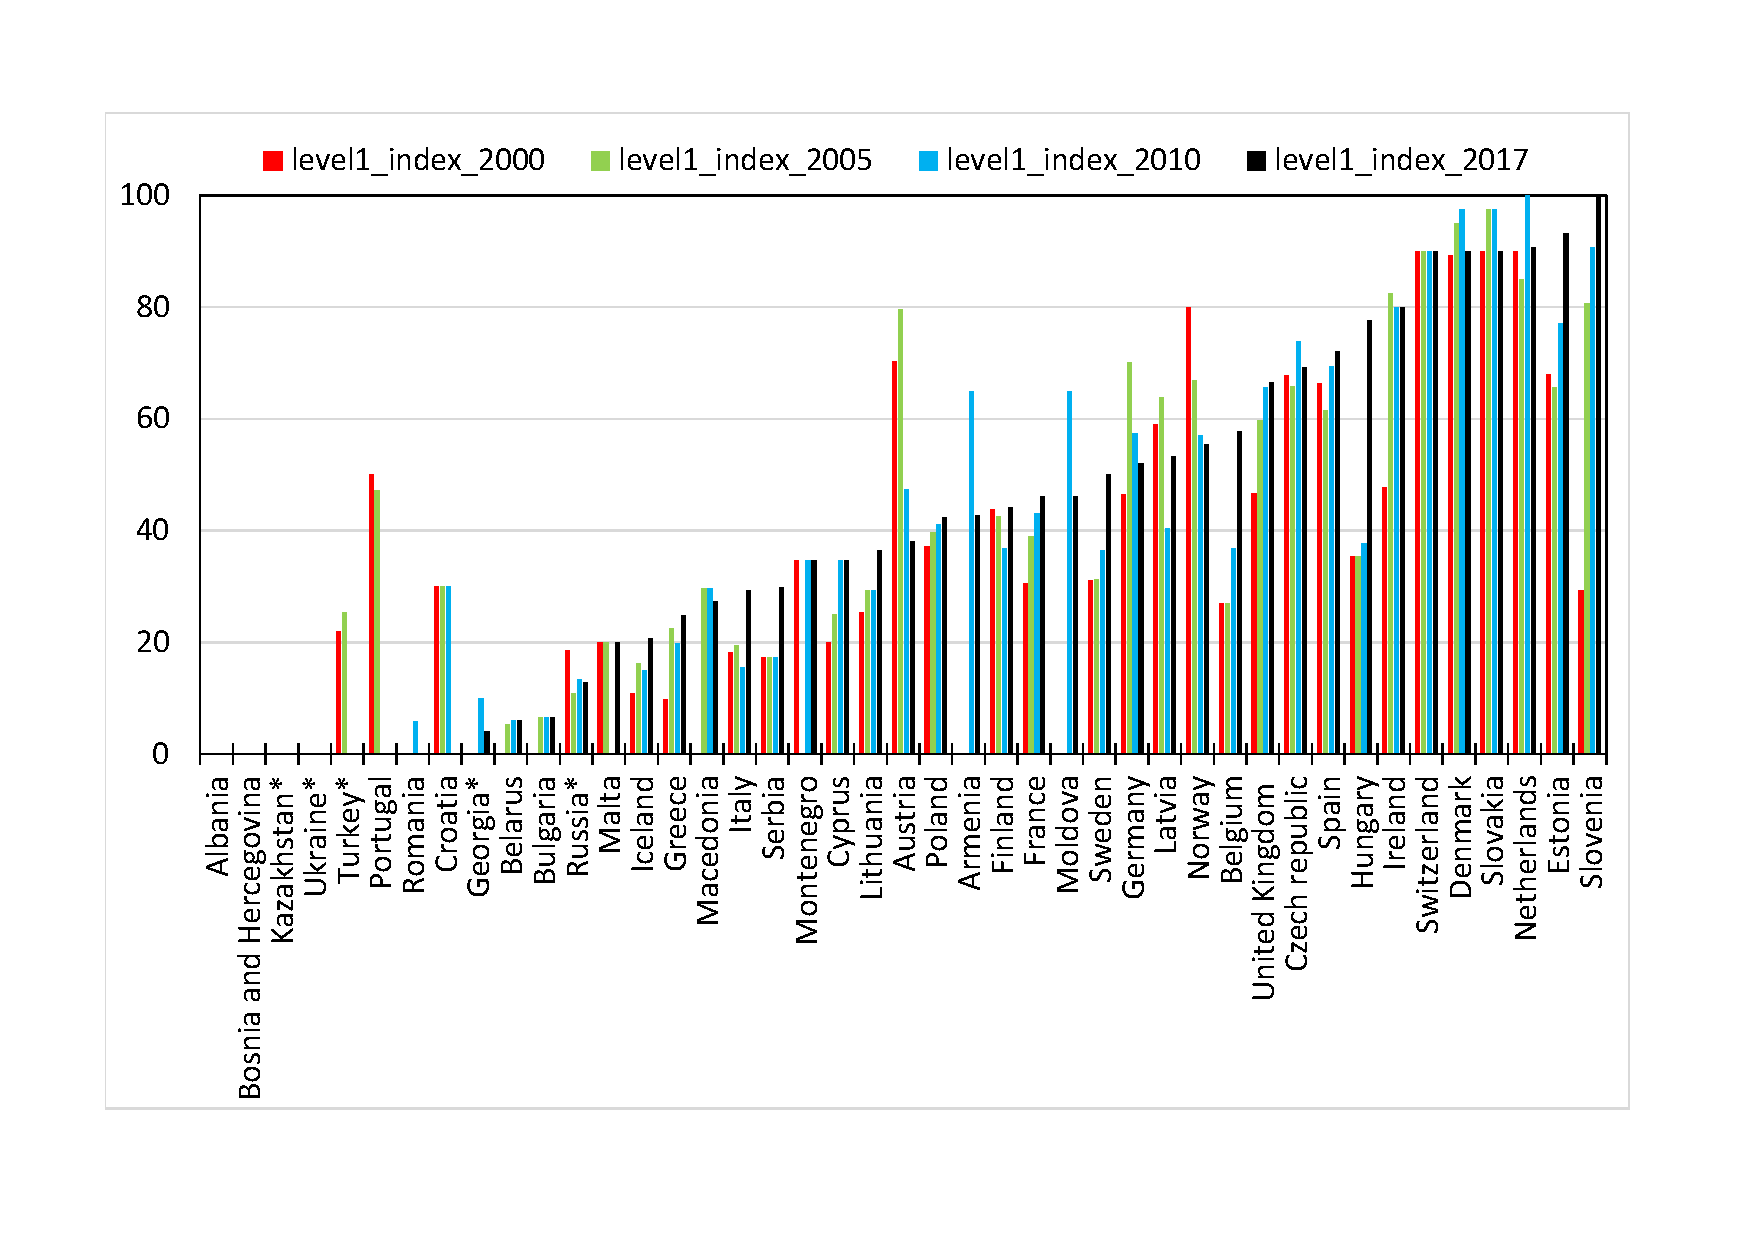
\includegraphics[width=0.74\paperwidth]{FIGS_Obs/index2017.pdf}
	\caption{\label{fig:Index-for-implementation}Index for implementation of the EMEP monitoring strategy, level 1 based on what has been reported for 2000, 2005, 2010 and 2016. {*} means adjusted land area.}
\end{figure}

For the level 2 parameters, an index based system has not been defined, but mapping the site distribution illustrate the 
compliance to the monitoring strategy. 45 sites from 18 different Parties reported  at least one of the required 
EMEP level 2 parameters relevant to this report (aerosols (36 sites), photo-oxidants (19 sites) and trace gases (9 sites)). 
The sites with measurements of POPs and heavy metals are covered in the EMEP status report published by MSC-E. 
Figure~\ref{fig:levell2-sites} shows that level 2 measurements of aerosols have better spatial coverage 
than oxidant precursors (VOC + methane) and trace gases. Few sites have a complete measurement program, 
and only 8 sites have a complete aerosol program. Nevertheless, regarding the aerosol monitoring, 
there have been large improvements in the spatial coverage and the data quality over the last decade. 
Standardization and reference methodologies have been developed, and the reporting has improved significantly 
with much more metadata information available. For oxidant precursors and trace gases, there are ongoing improvement in the measurement capabilities resulting from development in ACTRIS (Aerosols, Clouds, and Trace gases 
Research InfraStructure Network) and in co-operation with the WMO Global Atmospheric Watch Programme (GAW). 




\clearpage
\bibliographystyle{copernicus}         % change bibliography-name after each
\renewcommand\bibname{References}      % bibliographystyle command!
\addcontentsline{toc}{section}{References}
\bibliography{Refs,EMEP_Reports}
 %Wenche

%\part{Appendices}
\setcounter{part}{1}
\cleardoublepage
\setcounter{page}{1}
\begin{appendix}
\renewcommand{\theHchapter}{\Alph{chapter}}
\renewcommand{\thepage}{{\em page \Alph{chapter}:\arabic{page}}}
\renewcommand{\thepage}{{\Alph{chapter}:\arabic{page}}}
\renewcommand{\thetable}{\Alph{chapter}:\arabic{table}}

%\include{chapterAPPX_EMIS_2018}
%\include{chapterAPPX_EMIS_trends}
%\include{chapterAPPX_SR2018}
%\include{chapterAPPX_CountryRep}
%\include{chapterAPPX_ModelEval} % NEED TO INCLUDE AIRBASE? Michael G


\end{appendix}
\end{document}
